\documentclass[12pt,a4paper,oneside,openany]{book}

\usepackage{xcolor}
\usepackage[cache=false]{minted}
\usepackage{listings}
\usepackage[utf8]{inputenc}
\usepackage{tikz}
\usepackage{caption}
\usepackage{gensymb}
\usepackage{lmodern}
\usepackage{multirow}
\usepackage{booktabs}
\usepackage{array}
\usepackage{adjustbox}
\usepackage{upquote}
\usepackage{amsmath}
\usepackage{titlesec}
\usepackage[hidelinks]{hyperref}
\usepackage{fancyhdr}
\usetikzlibrary{mindmap,shadows, shapes, arrows, positioning}



%% Change these:
\newcommand{\projecttitle}{Videsign: A Real-Time Peer-to-Peer Web Conferencing Application With A Collaborative Whiteboard}
\newcommand{\projectauthor}{Connor Brookfield \\[0.2cm] Charlie Conneely}
\newcommand{\projectadvisor}{Gerard Harrison}
\newcommand{\projectprogramme}{B.Sc.(Hons) in Software Development}
\newcommand{\projectdate}{\today}
%% End of things to change.



\tikzstyle{rect} = [rectangle, fill=blue!50, text width=4.5em, text centered, minimum height=4em, rounded corners]
\tikzstyle{line} = [draw, ->, very thick]
\tikzstyle{oval} = [ellipse, fill=green!50, text width=5em, text centered]

\newcolumntype{x}[1]{>{\centering\arraybackslash\hspace{0pt}}p{#1}}


\begin{document}
  \begin{titlepage}
    \begin{minipage}[t][6cm]{\textwidth}
      \centering
      \rule{\linewidth}{0.5mm} \\[0.4cm]
      { \LARGE \bfseries \projecttitle \\[0.4cm] }
      \rule{\linewidth}{0.5mm} \\[0.8cm]
    \end{minipage}
    
    \begin{minipage}[t][6.5cm]{\textwidth}
      \centering
      \textbf{\projectauthor}\\[0.5cm]
      \projectprogramme
    \end{minipage}
  
    \begin{minipage}[t][1cm]{\textwidth}
      \centering
      \textsc{\projectdate}
    \end{minipage}
      
    \begin{minipage}[t][3cm]{\textwidth}
      \centering
      \textbf{Final Year Project}\\[0.3cm]
      Advised by: \projectadvisor \\[0.1cm]
      Department of Computer Science and Applied Physics\\
      Galway-Mayo Institute of Technology (GMIT)
    \end{minipage}
  
    \begin{center}    
      
\includegraphics{img/gmit-logo.jpg}
    \end{center}
  \end{titlepage}
  \setcounter{page}{2}
  \tableofcontents
  \listoffigures
  %!TEX root = project.tex

\chapter*{About this project}
\paragraph{Abstract}
Since the arrival of COVID-19, there has been a dramatic increase in the number of people working from home and subsequently in the necessity for web conferencing applications such as Zoom and Microsoft Teams. Previously, holding a meeting through video call was just one option, but for many, it is now the only option. With this shift towards remote conferencing, many tasks and activities now need to be performed using features provided by these video conferencing applications. Most notably, the ability to collaboratively sketch technical and/or business-related plans on a surface for all team members to observe. For these reasons, we have designed a peer-to-peer video conferencing application with a real-time, interactive whiteboard on which peers can visualise business ideas. Using React JS as the programming language, the HTML canvas element was used to render the graphical drawings which appear on the whiteboard. To fully utilise React JS, close attention was paid to the relevant features which it provides, and to the current trends and standards relating to JavaScript and ECMAScript. WebRTC was implemented to enable the application to capture, send, and receive microphone and camera data from within the web browser. For the backend, Socket.IO was used to establish the peer-to-peer connection and to enable the real-time, event-based communication of data. An additional goal of this project is to develop efficiently a software application in an integrated development environment using git and GitHub for version control, whilst exercising the best practices related to software development. 

\paragraph{Authors}
This project and dissertation was created by Charlie Conneely and Connor Brookfield, students of Software Development at the Galway-Mayo Institute of Technology.

\chapter{Introduction}
In recent years, the number of people working remotely has grown steadily thanks to evolving technological possibilities relating to web conferencing applications. However, during the coronavirus pandemic, that number has increased significantly as millions of workers were required to stay at home. This sudden paradigm shift meant that millions of students, workers, and businesses now require competent web conferencing applications such as Zoom, Skype, and Microsoft Teams to facilitate day-to-day tasks. Since January of 2020, Zoom has seen an increase of over 325 per cent in revenue~\cite{RichterZoom}. Although many will return to on-site working in time, it is likely that video conferencing will become more incorporated into all aspects of life as more people have now familiarised themselves with these technologies and recognised their usefulness.~\cite{samet2020coronavirus}  

As a result of this sudden move towards remote-working, we have seen an increase in the demand for workers with a particular skill set, who can not only maintain and develop these video conferencing applications, but who can also pioneer new and exciting features to facilitate a growing list of user needs. For these reasons, we will focus on the up-and-coming technologies which enable these applications to perform. Through developing an application which provides video-conferencing functionality, we can also push-forward the domain and ultimately make life as a remote employee easier.  

\section{Conferencing Systems}
\subsection{Background}
A conferencing system provides participants of different locations with a means of communication through the capturing, sending, and presenting of visual and audible data. In the beginning, we created video-conferencing systems for industrial use in business meetings in order to reduce travel costs and to save on various other expenses. In the 1980s, there were various forms of conferencing systems in circulation. The Single Person-Camera System (SPC) involved positioning one camera at an angle to be broadcasted to other participants. The Voice-Switched System (VSW) required one camera per person and an audio-triggered switch to broadcast the recordings of the speaker. Similar to what we would typically use today, the Continuous Presence System would broadcast and display all participants throughout the conference call. \cite{sabri1985video} Although these systems were groundbreaking in the 1980s, they were typically inconvenient, very expensive, and only feasible for industrial use. It was not until the mid-1990's that similar conferencing technologies reached the hands of the general public. 

In the early 1990s, video conferencing technologies reached the hands of the public with devices such as the CU-SeeMe. Developed by Tim Dorcey, the CU-SeeMe provided people with a simple conferencing system that only required a network connection, a gray-scale monitor, a camera, and a digitizer used to convert analogue media to computer-readable data. The device was first launched in multiple schools as part of a project, enabling students to connect with each other through the internet. The focus of the product was to teach the public about conferencing practices rather than to push forward the development of low-level features such as video compression.~\cite{dorcey1995cu} Since then, the accessibility, quality, and performance rates of video conferencing systems have improved drastically and as a result, have become commonplace. Applications such as Zoom, Skype, and Microsoft Teams take advantage of peer-to-peer internet technologies, combined with the availability of desktop cameras to provide millions with a high-quality conferencing system.    

\subsection{Structure}
There are three key components to a conferencing system:~\cite{firestone2007voice} 
\begin{itemize}
    \item \textbf{User Interface} – The front-facing part of the application with which the end-user will interact. From here, the user can enter a chat room in which they can communicate through audible and visual means with other participants, and interact with various other elements of the web page. 
    \item \textbf{Control plane} – The control plane connects peers together, handles the initial handshake, and manages incoming and outgoing messages.
    \item \textbf{Media plane} – Provides means of sending, receiving, and processing media streams such as audio and video. 
\end{itemize}

The traditional architecture for a conferencing system was Unicast or IP-Multicast. However, neither architecture is suitable for a modern web-conferencing application as Unicast is a one-to-one system, while IP-Multicast requires a specific network infrastructure and is not suitable for widespread commercial use. Peer-to-peer communication emerged as a far more suitable medium for audio and visual communication, as it does not rely on network infrastructure. Additionally, peer-to-peer communication allows for participants to handle the technical cost of receiving and parsing the incoming media stream whilst also uploading their own. These features greatly improve both the reliability and scalability of a conferencing system.~\cite{apu2017p2p} Socket.IO is an open-source library that enables applications to provide the end-users with peer-to-peer communication channels. Using a Node.JS server and the Mozilla WebSocket API, developers can establish event-based back end services to be triggered through client/browser-side activity.~\cite{arrachequesne_2021} Released in 2014, Socket.IO has become an incredibly popular tool used to provide an efficient means of peer-to-peer communication.  

WebRTC (Web Real-Time Communication) has become a popular tool to support the media plane, as it provides a simple, cost-effective means of obtaining media streams from the browser. Since WebRTC is an open web standard with a high browser compatibility rate, it is quickly becoming a key technology for conferencing applications.   

\section{Objectives}
The primary goal of this project is to develop a video-conferencing web application with an additional feature to facilitate business practices and clear communication. The purpose of the application itself is to enable peer-to-peer video and audio-based communication between two users. We provide both peers with an interactive whiteboard, on which they can sketch collaboratively. This digital whiteboard serves as a substitute for the typical surface available during an on-site meeting, on which team members can illustrate business ideas, such as a diagram depicting a project planning schedule or a software flowchart. 

When two peers connect in a virtual room, either peer should be able to take control of the whiteboard and draw on it. When one peer is in control, they should disable the whiteboard for the other participant, until the other participant hits the button to take control of the whiteboard for themselves. When a participant is in control, they should be able to draw on the whiteboard by left-clicking on its surface and moving the mouse whilst holding down the left-click. When they release the mouse click, the graphic should remain on the surface. All shapes rendered thereafter should be in addition to the previously rendered shapes. The user should also be able to undo individual illustrations or clear the entire whiteboard. To ensure usefulness in our application, we will provide an array of different shapes and graphics that one can choose to illustrate, all with a professional and artistic aesthetic.  

Throughout the development of this system, we aim to demonstrate clearly the implementation and usefulness of technologies such as WebRTC and Socket.IO. We will perform back-end programming with technologies such as Express and Node.JS. We will also implement various software packages using NPM for package management. Throughout the project, we will use React JS to demonstrate good programming practice through writing and maintaining readable, scalable, and reusable code. We will also exercise various key features which React provides, such as reusable components and React Hooks. We will develop our project using modern technologies that are recognised at an industry level. We will also uphold, throughout development process, the core principles of software design such as the DRY and SOLID principles. 

\section{Contents}
The contents of this paper are as follows.

\subsection{Chapter 1: Introduction}
\textit{Written by: Charlie Conneely} 
\subsection{Chapter 2: Methodology}
\textit{Written by: Connor Brookfield} \newline
We outline the different methodologies that we considered during our planning phase, which one we chose in the end, and why. 
\subsection{Chapter 3: Technology Review}
\textbf{Objectives} \newline \textit{Written by: Connor Brookfield} \newline
\textbf{Technologies} \newline
Introduction and Section \ref{backendservices} - \textit{Written by: Connor Brookfield} \newline
All other headings - \textit{Written by: Charlie Conneely} 

In this section, we outline our objectives and the technologies which would accommodate those objective most. We then talk, at a conceptual level, about the technologies which we chose to incorporate into our system, and why we chose them. 

\subsection{Chapter 4: System Design}
Section \ref{canvas-component} - \textit{Written by: Charlie Conneely} \newline
Introduction and All other headings - \textit{Written by: Connor Brookfield} 

Here we discuss how we utilised the technologies outlined in the Technology Review. We also illustrate the structure and inner workings of our application at a high and low level.

\subsection{Chapter 5: System Evaluation}
Section \ref{selenium} - \textit{Written by: Connor Brookfield} \newline
All other headings - \textit{Written by: Charlie Conneely} 

Here, we will outline what was accomplished during development. We will also discuss the applications robustness with regard to Acceptance Testing and the use of Selenium IDE. Finally, we will discuss the shortfalls of the application and the reasoning for these.

\subsection{Chapter 6: Conclusion}
\textit{Written by: Charlie Conneely} \newline
Here, we will summarise the objectives of the undertaking, what was accomplished, discovered, and discuss potential future work. 

\subsection{Source Code URL} 
The GitHub repository for this project can be found at the following address: \href{https://github.com/charlieconneely/final-year-project}{https://github.com/charlieconneely/final-year-project}. \newline 
The main elements of the repository are as follows.
\begin{itemize}
    \item A \textbf{src} folder containing all of the source code for the application. 
    \item The \textbf{server.js} file contains all the back end, server-side code which manages the initial Express/Socket.IO setup, and specifies all the Socket.IO P2P functionalities such as event-handling, and data broadcasting.    
    \item A \textbf{package.json} file which manages all of the project dependencies and versioning. 
    \item A \textbf{README} markdown file with which briefly describes the application, and provides instructions for installation, compilation, and running the program.  
\end{itemize}

\chapter{Methodology}
\section{Developmental Approach}
For the methodology undertaken for the project’s development, we took a look at an array of different developmental approaches before making a decision on which specific approach to take. 
There are six main agile developmental methodologies: crystal methodologies, the dynamic software development method (DSDM), feature-driven development, lean software development, extreme programming and scrum \cite{dybaa2008empirical}. 

Within crystal methodologies (a family of the methods: Clear, Orange, Yellow, Blue and Read), we took a look at the crystal method. This development methodology requires the first three of the seven principles to be considered Crystal Clear; frequent delivery, reflective improvement, osmotic communication, personal safety, focus, and a technical environment with automated tests, frequent integration and configuration management \cite{cockburn2004crystal}.

The Dynamic Software Development Method (DSDM) consists of three project phases: the pre-project phase, the project life-cycle and the post project phase. The nine principles of the Dynamic Software Development Method include: active user involvement, project team empowerment, frequent delivery, accepted deliverable for business needs, iterative and incremental development, reversible changes (due to changed priorities in given requirements), high-level requirements are baseline, testing throughout the project life-cycle, and effective and collaborative communication \cite{voigt2004dynamic}.

Feature-driven development is a feature-centric process that retains agile motivations. A feature centric process is a development process that combines the units of requirement with the units of planning and work, so that features a user wants can be planned, monitored and used as a form of work allocation. The key aims of this approach (while retaining agile’s original motivations) are to: satisfy the customer’s needs, deliver working software that provides value to customers, primarily measure the progress of a project through the software’s ability to work, promote sustainable development and to keep project processes as simple as possible \cite{hunt2006feature}.

The Lean software development methodology features five core principles within its customer-centric software development life-cycle. These elements include: creating value for a customer, eliminating/reducing overhead, project team empowerment, work stream efficiency, and continuous improvement \cite{ebert2012lean}.

The Scrum methodology has three groups of development phases: pregame, game, and postgame. The pregame development group consists of a planning phase and an architecture/high level design phase. The game group consists of a development or “Sprint” phase, which is an iterative development cycle and set of development activities that one or more teams can perform: develop, wrap, review, adjust. After the sprint, a review is held, and if the project manager(s) feel that the projects requirements, cost, time, quality and competition are up to their standard, development will move onto the postgame development phase which prepares the software product for general release \cite{schwaber1997scrum}.

We decided to go with feature-driven development as it appeared to be the most suited for the project idea we had prepared. The iterative nature of the development of each feature appealed to our project, as the main focal point of the project were the development of individual features such as the canvas feature and the video features.

\section{Project Requirements}
Before researching and deciding on a development methodology, we had to come up with an idea for a project. When the assignment was declared, our team organised weekly meetings to brainstorm project ideas. Our original project idea was to create a mobile application that can read text on a surface using the phones camera, and translate the text to a desired language. We researched the technologies we would use for this project including react-native and google translate and text detection APIs. Upon planning time management and discussions with our project supervisor, we came to the realisation that using the Google Translate API and the Google Text Detection API would be relying too heavily on external APIs and that we would have to manually develop the functionality of one of the APIs. This proved to significantly skew the time management of the project due to the development cycle predicted to take too much time.
After this, we pursued another idea that we brainstormed. We thought of creating an application that could translate on screen text from a video or stream in real-time to the user’s chosen language. Upon sharing this idea with our project supervisor, we were informed that the scope of the idea reigned too large in relation to our time management for this project.

Failing the previous idea, we continued brainstorming, and arrived at the idea of creating a web conferencing application with a shared virtual canvas. Our desired idea for the dissertation project was to create a project that could provide value in communication to someone. During the scheduled weekly meetings within our project team, we decided upon creating a peer to peer web conferencing application with the second main feature being an interactive shared whiteboard. The requirements for the project were discussed throughout the weekly meetings, and were decided on based off of the time required to conduct the research, development, integration and testing of the individual features.

\section{Testing}
For the testing of this web application, we decided to use Selenium. Selenium was decided on as the testing tool of choice during the weekly meetings, as it is used widely to automate tests within a web browser \cite{gundecha2012selenium}. The automation of test cases proved very intuitive as they became accessible to write and rerun when a change was required in the code and it needed testing again to make sure that no bugs had been introduced before pushing it from the feature branches to the main development branch. We tested the web application on both Firefox and Google Chrome on Windows, Linux and Android OS.

\section{Tools}
Initially during brainstorming sessions at weekly meetings, our team discovered that we would like our project to ultimately comprise of JavaScript, Node.js and the React framework, due to their rising popularity and use within leading brands and projects \cite{borges2015popularity}. 
When conducting the research for this project and presenting our ideas during weekly meetings, we discussed and decided on several developmental tools that would be beneficial during the development of this project. For coding the JavaScript side of the application, we came to the mutual agreement that Visual Studio Code would be our coding environment due to it being lightweight, fast and extensive language support due to the multitude of Microsoft and community developed extensions readily available to make coding JavaScript applications more intuitive.

We decided to develop the application using two different web browsers where one party used Firefox and another used Google Chrome. This decision was conducted to make sure that our web application would support the most popular and widely used web browsers and could work also work cross platform with Linux and Android users.

\subsection{Version Control}
It was a discussed decision that we would use GitHub as our version control software. We have been using it extensively during our time in college, it is a popular system, efficient, and an easy way for us to manage our code, versions and feature development.

To ensure efficient coordination during the development of our project, we utilised git branching. By creating a separate branch to the default main, we can develop code and push to our remote repository without affecting the main branch. We took this approach because it is common practice in the software industry to only develop software on a separate branch, and to only merge a stable version of the project back to main. 
Below in Figure \ref{branchingDiagram}, we can see the manner in which we branched our git repository. From main, we created a development branch, and from here we created a further two separate branches; one for the development of the canvas or whiteboard area of the system, and another for the video chat component. Separating our work spaces in this way allowed us to develop our own features locally with the assurance that the remote branches were unchanged. When we had crossed a significant milestone in our development, we would both merge back to the development branch and fix any resulting conflicts. Finally, when we were confident that we had created a fully stable version of the project, we would merge from the development branch back to main.   
\begin{figure}[H]
    \centering
    
\includegraphics[scale=0.4]{img/flow-chart.png}
    \caption{GitHub branching structure.}
    \label{branchingDiagram}
\end{figure}

\section{Empirical Experience}
An empirical approach was somewhat taken at the start of this project. For the video feature, the idea of creating a peer to peer video stream was hard to conceptualise theoretically, so an external library called “Peerjs” was used. Although the feature did not work initially, “Peerjs” became a foundation for related research into understanding the concepts of peer to peer based networking and media streaming. This helped the transition from an empirical approach to a more theoretical one, which in turn make the development process easier when developing the feature from scratch using the WebRTC functionality built into the standard JavaScript library without the use of the “Peerjs” Node.js library.

\chapter{Technology Review}
\section{Objectives}
\label{objectives}
As outlined in the introductory chapter of this dissertation, the objectives our team had brainstormed over the course of weekly project meetings for this project, includes: 
\begin{itemize}
\item Developing a video-conferencing web application with additional features to facilitate business practices and clear communication.
\item Enabling video and audio-based communications between two peer-to-peer clients.
\item Providing users with a collaborative whiteboard to share and visually communicate ideas.
\item Utilising the SOLID design principles in our application to ensure that our code can remain scalable, reusable and easy to maintain.
\item Demonstrating independent learning through utilising features we have not previously used in technologies that our team is familiar with.
\end{itemize}

\subsection{Developing a Video Conferencing Web Application}
Upon brainstorming ideas at the project team’s weekly meetings, we came up with the idea of developing a video-conferencing web application with additional features that could be used to facilitate business practices. This particular idea struck a chord with us due to the rise of web conferencing systems among businesses and the general public as a result of physical conferencing and mingling of citizens being banned due to constraints on the movement of non-essential workers as a result of the global Covid-19 pandemic \cite{hacker2020virtually}. 

In terms of additional features, our project team settled on a collaborative virtual/interactive whiteboard as it has a place in a physical conference when presenting ideas, training groups of people, and collaborating with clients and colleagues in real-time, due to its ability to become a clear method of communication when a user knows how to effectively convey information through that commonly used medium.

This objective has been achieved and effectively implemented due to the careful planning, organisation, weekly meetings and vigorous testing of our project team and the modern technologies that our project team had decided to use for this project. The collaborative whiteboard has fulfilled the role of the additional feature used to facilitate common business practice and to provide an alternative method of clear communication for this video-conferencing web application.
\subsection{Enabling Video \& Audio, Peer to Peer Communications}
During one of the many weekly meetings, the project team presented an argument about modern video conferencing applications do not use peer to peer communication when conducting conference calls between two or more users. This was a valid argument largely due to the fact that peer to peer communication involves users sending their video feed directly to the other peers, which would not be efficient in a large conference due to bandwidth limitations on the individual users having to stream their audio to each individual instead of sending their video stream directly to a server, that would then be broadcast to the other participants in the video conference. 

For our project, peer to peer communication was decided upon by the project team due to the number of users being limited to two per call because of time constraints within the project. This method proved ideal between two participants, for several reasons, one of which being the privacy involved. Peer to peer communication grants the participants of a call more privacy than a more traditional method, due to the users sending video and audio streams directly to the other users instead of sending the content to a server in the middle to distribute it between the users. This project goal was achieved and implemented using the WebRTC API within the standard JavaScript library.
\subsection{Providing a Collaborative Whiteboard}
To visually communicate and share ideas, both as a business feature for video conferencing and as a recreational collaboration tool, our project team had succumbed to the idea of producing this feature as an interactive and collaborative whiteboard. It is a fun way of communicating between individuals through the medium of art and self-expression, but it is also an important teaching tool and a meaningful way to visually transmit, present, and collaborate important information between groups of people. 

We chose a virtual and collaborative whiteboard as the main alternative way of communication for this project, specifically for those reasons and for another logical reason. In one study conducted over 170 classrooms and 85 teachers in 2019, statistics from that study informed our project team, that teaching a class using an interactive whiteboard is an effective way for students to learn new material, as the results of the research found that in general within student achievement, that there was a “16 percentile point gain in student achievement” \cite{ marzano2009teaching}. This intrigued our project team and presented us with another important reason to implement an interactive and collaborative whiteboard into our web conferencing video application. 

The concept of the collaborative whiteboard objective for this project was achieved and was successfully implemented into this project using the HTML5 Canvas Element, Socket.IO, and JavaScript using the React framework.
\subsection{Utilising SOLID Design Principles}
While discussing the software design principles to be undertaken when designing the software architecture of the program during the weekly meetings between our project team, a new objective for this project was set. This objective was to adhere to the guidelines present within the “SOLID” software design principles, as they present us with good advice for a programming paradigm as having knowledge of various principles and patterns may not make us fantastic programmers, but when understood, it will provide us with the justification and wisdom to apply them, which in turn would make us good programmers \cite{martin2013getting}. “SOLID” is an acronym for a multitude of software design principles. The “S” in “SOLID” stands for the “Single Responsibility Principle”, the “O” represents the “Open Close Principle”, “L” is an abbreviation of the “Liskov Substitution Principle”, the “I” represents the “Interface Segregation Principle” and the “D” in “SOLID” makes reference to the “Dependency Inversion Principle”.

Our project team has effectively followed the “SOLID” design principles throughout our project, which has resulted in our code being predominantly reusable, scalable and easy to maintain, which was one of our biggest objectives while carrying out this project, as it insures that if any members of our project team choose to carry out a similar project, the code could be reused in that project and it would retain its ability to be easily maintainable and scalable. 

\subsection{Demonstrating Independent Learning}
During the weekly project meetings between the project team, we discussed the learning outcomes we expect to achieve over the course of the development of the project. In terms of programming, one of the learning outcomes was to become familiar with technologies the project team have not used before such as the JavaScript WebRTC and Canvas APIs. Another outcome was being able to manage an Agile project. This was initially a lot harder than our project team had anticipated, largely due to a mismanagement of time at the start of the first semester for brainstorming project ideas and the development of project features. Our project team got into the workflow of managing our team effectively and conducted a set schedule for the development of various crucial features, testing, front end development, and the write up on the dissertation to compliment the project.

When initially undergoing the development of the video streaming feature, our project team became quickly acquainted with some crucial issues regarding the approach undertaken to access and transmit client data to the other parties using the PeerJs JavaScript API installed from the “Node Package Manager” also known as “NPM”. This approach was soon after deprecated and another approach utilising the WebRTC API from within the standard JavaScript library and the Socket.IO API (also downloaded and installed using NPM). This new-fangled approach involved the project team replicating the functionality of the PeerJs API (of which uses the WebRTC package and presents the developer with a higher-level use of the WebRTC technology), using the WebRTC package. This provided our project team the invaluable opportunity to learn about the way in which real time communication between multiple parties is conducted and works at a lower level, in contrast to the use of the PeerJs API with its higher level overview of real time video and audio communication.

I think the objective of our project team to demonstrate our ability to independently learn a multitude of learning outcomes ranging from project management from an Agile standpoint, to learning how to develop web applications with a new approach utilising different packages and technologies, has been successfully accomplished.

\section{Technologies}
Our project team’s choice of technologies to use for the development of this project have been for the most part empirical. Throughout our four years in college, our project team has been using JavaScript from the first year, and the consecutive years spent constantly progressing our programming experience in that domain, through development using various frameworks such as Angular and React (of which the latter, we have spent two years developing with). JavaScript as a result became a preferred scripting language when brainstorming ideas behind the project we should undertake for our final year and React being the preferred JavaScript framework for that project. The React framework is a JavaScript framework that works with JavaScript, HTML, CSS, and styling APIs for styling various elements, which proved to make development for this project easier than the traditional method of creating a HTML page, using an external JavaScript script and creating multiple CSS files.

When the project idea had been decided upon, our project team initially did not know which packages to use to carry out the functionality required for the web application project, but we knew  that our package manager of choice would be Node Package Manager (also known as NPM) due to its use with JavaScript over the course of our college tuition. The packages for use with this project were also decided empirically, as we made a list of potential package options that could be used for certain functionalities such as the Graphical User Interface (also known as GUI) styling, peer to peer networking, sending and receiving video and audio streams, back end server development in JavaScript, and real time event based communications. This list of potential packages would serve as a stack in which we would try each package, experiment with it, and remove it from the list if it was not the package/API that best suited our needs for that feature.

\subsection{Languages}
\label{languages}
\subsubsection{React}
React is a JavaScript library for building user interfaces.~\cite{reactjs} Facebook developed React in 2011, and it is currently the dominant JavaScript programming library. React provides a fast and interactive way to develop web applications with the traditional three key languages: Hypertext Markup Language (HTML), JavaScript and Cascading Style Sheets (CSS). By using React, developers do not have to worry about managing the Document Object Model (DOM) through a browser’s DOM API. React will create a virtual DOM based on our application and map this to the real DOM. Any changes made to the state of the virtual DOM will cause an automatic update of the real DOM, hence the name “React”.  

A key feature of React is that it is component-based. A typical React application comprises multiple components which are nested amongst each other. A React app is essentially a component tree with a single component at the root. Typically, we call this root component "App".    

\begin{figure}[H]
    \centering
    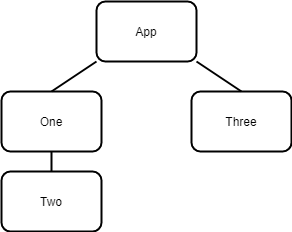
\includegraphics[scale=0.5]{img/TechReview/ReactComponents.png}
    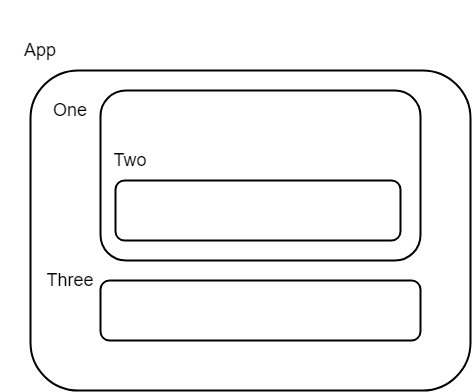
\includegraphics[scale=0.4]{img/TechReview/web-components.png}
    \caption{React component tree and it's appearance on the UI}
\end{figure}

To develop the component tree seen above, we first would have to create each individual component. The code snippet below illustrates how we can create, import, and nest a component.    

\begin{minted}{javascript}
// import the react library
import React from 'react'
// import component to be nested 
import Two from './two'

// define component
const One = () => {
    // HTML element 
    return (
        <div>
            <h2>One</h2>
            <Two />
        </div>
    )
}
// export component
export default One
\end{minted}

Finally, we need to nest all of our components in the root App component. 

\begin{minted}{javascript}
// import our components
import One from './one'
import Three from './three'

function App() {
    return (
        <div>
            <One />
            <Three />
        <div>
    )
}
export default App
\end{minted}

By using React components, we can isolate parts of our application for reuse and ultimately contribute to a far more maintainable and scalable application. React is also a language that relies heavily on dependencies, so by using React, we have more freedom to select the dependencies which we believe would benefit our system most, whilst further familiarising ourselves with package management systems.

\subsubsection{Sass}
Sass (Syntactically Awesome Style Sheets) is a powerful style sheet language written in Ruby that is compiled to raw CSS. \cite{sass} 
Sass provides a way to develop CSS code using variables and \textit{mixins}. Mixins act as a template for a specific collection of styling features. These features are extremely useful as with CSS, we often have to repeat chunks of code for various classes which have slight variations from each other. For example, in the code snippet below, we can see an instance in which we would be forced to repeat ourselves using raw CSS. 
\begin{verbatim}
.topSection {
    background-color: #ffffff,
    padding-left: 5%,
    padding-right: 5%
}

.bottomSection {
    background-color: #ffffff,
    padding-left: 4%,
    padding-right: 4%
}
\end{verbatim}

The code above is in direct breach of the DRY programming principle (Don't Repeat Yourself). For both classes, we were forced to specify twice the features which we want to define (background colour etc.). We also had to specify the background colour twice. However, using Sass, we can define a variable for the colour, and a mixin for reuse in both classes. 

\begin{verbatim}
// variable definition 
$bgColour: #ffffff;
// mixin for reuse 
@mixin colourAndPadding($colour, $pLeft, $pRight) {
    background-color: $colour,
    padding-left: $pLeft,
    padding-right: $pRight    
}

.topSection {
    @include colourAndPadding($bgColour, 5%, 5%);
}

.bottomSection {
    @include colourAndPadding($bgColour, 4%, 4%);
}
\end{verbatim}

Above, we maintained the DRY principle by referencing variables and by passing our class-specific values into a mixin as parameters. Thanks so Sass, the code is also now easier to modify and extend. 

\subsection{Back End Services}
\label{backendservices}
\subsubsection{Express JS}
Express JS is a fast, flexible minimalist web framework for Node JS. This technology can be used to create back-end/server-side JavaScript applications and robust, quick, and easy APIs. An express application can be created using a minimum of two JavaScript lines, as shown below in Figure 3.2.

\begin{figure}[H]
    \centering
    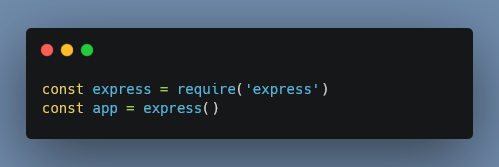
\includegraphics[width=0.8\textwidth]{img/TechReview/expressJs.png}
    \caption{Getting started with Express JS. Image created using \href{https://carbon.now.sh/}{\textit{Carbon}}.}
\end{figure}

\subsubsection{Socket.IO}
Socket.IO is a JavaScript library that allows developers to use real-time and event-based bidirectional communication between a browser and a server. To use Socket.IO, a Node.JS/Express JS, Java or Python server is required for the server side events, and a Socket.IO client-side library (which can be downloaded and installed using Node Package Manager, also known as NPM). Much like the server-side implementation of Socket.IO, Socket.IO has multiple client-side implementations in various programming languages other than JavaScript, including: Java, C++, Swift, Dart, Python, .Net, Golang and Rust.

Socket.IO is like WebSocket but it is not a WebSocket implementation. It uses WebSockets to transport data, but a WebSocket server or client would not be able to communicate with a Socket.IO server or client, due to Socket.IO adding extra metadata to each packet being transmitted. In comparison to WebSocket, Socket.IO is more reliable due to the ability to fallback to HTTP long-polling if a WebSocket connection cannot be made and automatically reconnect. It also allows servers and clients to broadcast to all clients or a group of clients by use of what the Socket.IO team call a “room”.

\subsubsection{WebRTC}
WebRTC is an open-source JavaScript project that allows high quality real-time communications (also known as RTC) to create browser and mobile applications using APIs and direct peer to peer communication. This project widely supported by companies such as Apple, Google, Microsoft, Mozilla, and Opera, which allows for their respectively major browsers to be compatible with the technology, without user’s having to install plugins for the services to work. 

Common applications of the WebRTC project, is the transmission of video streams, audio streams, text, and generic data between clients for real time messaging, video conferencing, and audio applications. Many popular modern applications such as Facebook’s Messenger, WhatsApp, Instagram, Telegram and Google Hangouts utilise WebRTC for their real-time communication services.


\subsection{Tools and Dependencies}
\subsubsection{HTML5 Canvas Element} 
\label{canvasSection}
Created by Apple in 2004, the canvas element was included as a feature of HTML5. It provides developers with a tool for creating and displaying graphics on the HTML document. To gain access to the canvas element via JavaScript code, we use the getElementById method. From here, we can call the getContext method on the canvas object and save its returned value to a variable traditionally called “context” or “ctx”. Once we have the context variable, we can begin using various methods to render graphics on the HTML document.  

\begin{minted}{javascript}
var canvas = document.getElementById("canvas")
var ctx = canvas.getContext("2d")
ctx.fillStyle("rgb(10,10,10)") // fill canvas colour
\end{minted}
\begin{minted}{html}
<canvas id="canvas" width="150" height="100"> 
    Fallback message for incompatible browsers. 
</canvas>
\end{minted}

To position graphics on the canvas, we need to provide an x and y coordinate. All coordinates are relative to the (0,0) position, which is at the top left of the canvas element.  

The only primitive shape supported by the canvas element is a rectangle. For the creation of these shapes, the canvas element provides functions which take in parameters and coordinates.  

\begin{minted}{javascript}
// params: x, y, width, height
ctx.fillRect(20, 20, 70, 60)
\end{minted} 

We must create all other shapes using individual lines by specifying the coordinates of shape corners and by drawing paths between each of these. The following code snippet will draw a triangle. 

\begin{minted}{javascript}
// define new path 
ctx.beginPath()
// start at pos x, y
ctx.moveTo(150, 100)
// create a line from here to start pos
ctx.lineTo(200, 150)
// create a line from here to last pos
ctx.lineTo(200, 50)
// fill area
ctx.fill()
\end{minted}

Although HTML Canvas is a very interesting and useful development tool, it does not provide any extra functionality beyond the rendering of specified graphics. Unlike other elements on the HTML document, we do not have any means to reference or manipulate shapes that are already rendered on the canvas bitmap. To implement a collaborative whiteboard using the HTML canvas, we need to save all rendered shapes as JSON data to be communicated, parsed, and re-rendered by all connected peers. Using the basic functionality exposed by the JavaScript Canvas API and by the HTML5 canvas element, designing an application which can render, maintain, and communicate a wide range of shapes would be a cumbersome task, and would ultimately produce a system with low scalability and readability. For these reasons, the canvas element and JavaScript Canvas API will serve as the foundation for our collaborative whiteboard. For further development, we will implement the JavaScript library Rough JS, the details of which are outlined below.   

\subsubsection{Rough JS}
\label{roughSection}
Rough JS is a JavaScript library that provides developers with a simplified way of creating various shapes on the HTML canvas element with a sketchy, hand-drawn style.~\cite{shihn2019rough} Since the only primitive shape supported by the canvas element is the rectangle, Rough JS is extremely useful as it exposes methods to draw a variety of shapes such as circles or ovals.

To set up the Rough JS library in JavaScript code and associate it with the canvas element, we must pass our canvas object to the Rough JS object as follows. 

\begin{minted}{javascript}
// import Rough JS package
import rough from 'roughjs/bundled/rough.esm'

// inside react component 
var canvas = document.getElementById('canvas')
var roughCanvas = rough.canvas(canvas)
\end{minted}
To produce a shape, Rough JS provides a generator object. From here, we can call functions to create a shape or a simple line by passing in coordinates as parameters.  

\begin{minted}{javascript}
const generator = rough.generator();
var element = generator.rectangle(10, 20, 20, 30) // x1, y1, x2, y2
// render the shape on the canvas 
roughCanvas.draw(element)
\end{minted}
The generator object also allows for extra parameters to be passed in, including dynamic CSS styling.

\begin{minted}{javascript}
var element = generator.rectangle(1, 2, 3, 4, {
    fill: "red",
    strokeWidth: 5
})
\end{minted}
Since the generator returns an object which the draw function can understand, we can now store multiple shape objects on the state array of our React application. To render these objects, we simply have to loop through this array and pass each object into the draw function. In our application, we keep a state array called \textit{elements} which stores all of our shapes, we can parse this array onto our canvas as follows.

\begin{minted}{javascript}
elements.forEach(e => {
    roughCanvas.draw(e);
})
\end{minted}

Since we store these shape objects as JSON data, we can also communicate them effectively between peers. 

The artistic shapes which this library provides ultimately contributed to a more visually pleasing graphical user-interface. Also, by streamlining most of the low-level programming associated with the HTML canvas element, we have created more readable code. 

\subsubsection{Create React App}
An official, supported way for anyone to bootstrap a React application without having to perform any manual configuration. By running “npx create-react-app AppName”, we can create a skeleton React application with built-in features such as a live development server, and basic unit-testing functionality. By initialising our application with Create React App, we are ensuring stability from the offset.   
\subsubsection{Material UI}
A JavaScript library that provides pre-made UI components, such as buttons and input fields. Material-UI components are designed with front-end best practices in mind and with close attention paid to typography. By incorporating Material-UI, we can guarantee modern and professional-looking components for our application's user interface. 
\subsection{Dependency Management}
\subsubsection{Node Package Manager}
\label{npm_section}
Released in 2010, Node Package Manager (NPM) is currently the primary software package manager for JavaScript and is the default package manager for Node.js.  
In short, package managers like NPM prevent developers from being forced to reinvent the wheel during development. Rather than developing every aspect of the application from scratch, using NPM, we can take advantage of a massive open-source library of community-developed software packages. Many popular NPM packages are maintained and developed publicly on GitHub. Since NPM is the most popular JavaScript package management system, we are familiarising ourselves with a modern, industry-standard technology.     

\subsection{Version Control}
\subsubsection{Git}

Git is an open source distributed version control system created in 2005. When we initialise a Git repository within a folder, it will continually track any changes made within that folder. When we add a feature and it works properly, we can run the following command in the command line.  

\begin{verbatim}
git add .    
\end{verbatim}
  
This will add all changes made to any files to the index. The index refers to the state of the application that we would like to commit eventually.~\cite{loeliger2012version}   

A commit represents a single version of the entire project. Every time we stage a commit, we add that version of the project to the commit history and assign it a unique ID, as well as information about the developer. During development, we should stage a commit after adding a significant change or feature and attach a descriptive commit message. It is important to commit continuously throughout development as it gives us the ability to revert to a specific version of the project if necessary.  To stage a commit, we must execute the following command. 

\begin{verbatim}
git commit -m "Descriptive message of the changes made"    
\end{verbatim}
 
To push the state of our local repository to a remote repository, we execute the following command. 

\begin{verbatim}
git push  
\end{verbatim}

Git is an important tool to use during development as it helps us to track bugs and enables us to save multiple versions of a project at a minimal cost.      

\subsubsection{GitHub}
Founded in 2008, GitHub is a web application for hosting Git repositories. By using GitHub, we can share, maintain, and collaborate on projects together. It provides all the functionality of Git along with extra features such as access control and bug-tracking, all delivered through an intuitive graphical user-interface. GitHub is an essential tool for collaborative development, as it provides a platform on which team members can both coordinate and examine each others' work. 

\subsection{Development Environments} 
\subsubsection{Visual Studio Code}
We developed our application source code using VS Code as it is a powerful code editor that inflicts minimal stress on the operating system. VS Code is lightweight because it is the developer's responsibility to install the necessary extensions from their open-source library. This characteristic is favourable, as it allows us to be more aware of the inner workings of the software system. Developing software in this environment is fitting because it reflects React as a programming language, which also promotes active involvement regarding package management.   

% === SYSTEM DESIGN SECTION === %

\chapter{System Design}
Upon finalising our decision of our final year project idea, our project team’s attention had been set upon discussion and planning behind the architectural design of the software project. Our project team’s key goal was to create the web application utilising the best programming practices to our knowledge, to promote as many as the SOLID principles as possible.

\section{Architecture}
Architecture or the structure of software is a critical aspect of design for software products and remains a staple in the design of large or scalable applications \cite{garlan1995introduction}. In Figure \ref{high-level-diagram} below, there is a high level diagram that illustrates the relationship between the React, Canvas, WebRTC, Socket.IO on the client side connecting to the server to point the clients in the direction of each other ultimately bypassing the server once the connection between the two clients has been determined.

\begin{figure}[H]
    \centering
    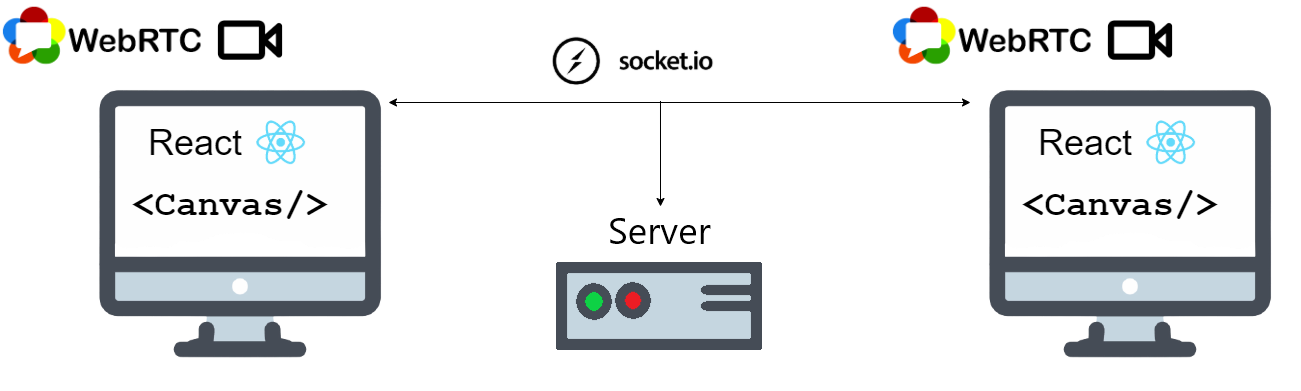
\includegraphics[scale=0.4]{img/arc-diagram.png}
    \caption{High level diagram.}
    \label{high-level-diagram}
\end{figure}

Outlined in the following sections are the various components that are crucial to the architecture of this project. The relationship between each of the components used throughout this final year software project is displayed in the architectural diagram below in Figure \ref{architecuralDiagram}.

\begin{figure}[H]
    \centering
    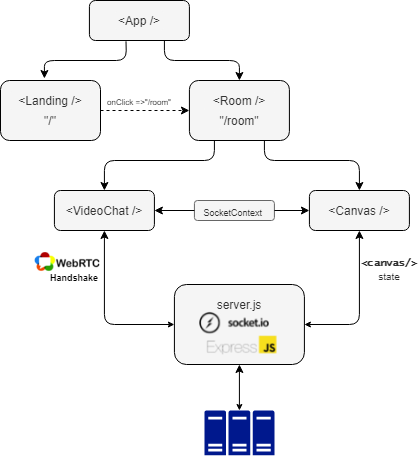
\includegraphics[scale=0.8]{img/SystemDesign/full-architecture.png}
    \caption{Architectural diagram.}
    \label{architecuralDiagram}
\end{figure}

The entire component tree for our applications front-end can be found below in Figure \ref{full-comp-tree}.

\begin{figure}[H]
    \centering
    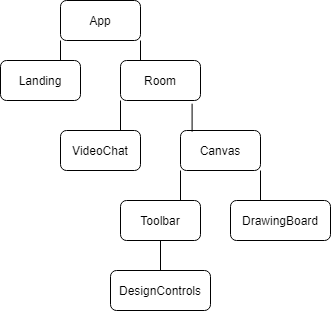
\includegraphics[scale=0.7]{img/SystemDesign/full-component-tree.png}
    \caption{Entire Front-end Component Tree}
    \label{full-comp-tree}
\end{figure}

\subsection{React components}
The foundation in which this project has been built upon is the React JavaScript framework. The functionality of this framework, as outline in Section \ref{languages}, allows for multiple JavaScript classes and functions, and higher abstraction due to multiple files. This section covers the various JavaScript files that are present for the operation and navigation of the React application but excluding the main features such as the video chat component, canvas component, cascading style sheets and the server back-end.

\subsubsection{Index.js}
This JavaScript file, which is a part of the React Framework, is called as a script file by the index.html. The index.html page is the first file to be loaded by the browser. Inside this Index.js JavaScript file, it creates an instance of App.js, and defines it as the root of the application, as shown below in Figure 4.3.
\begin{figure}[H]
    \centering
    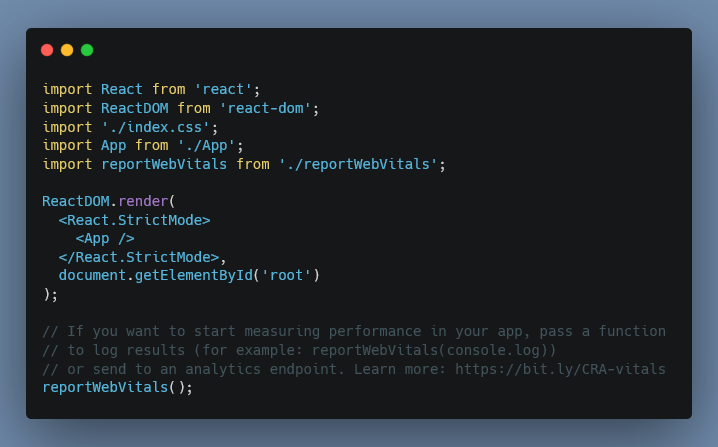
\includegraphics[width=0.8\textwidth]{img/SystemDesign/indexJs.png}
    \caption{Index.js, source code. Image created using \href{https://carbon.now.sh/}{\textit{Carbon}}.}
\end{figure}

\subsubsection{App.js}
The App.js JavaScript file is the root of the React Framework for JavaScript files. App.js creates global URL routing paths from various components and classes that have been imported from various JavaScript files. In the instance of this project, the components that are imported include: “VideoChat”, “Canvas”, “Room”, “Landing”, “SocketContext” and “io”. These components have global URL routing path extensions for the application to allow the user or application to navigate to different components throughout the application, by adding the appropriate relative path to the root URL.

The “io” component in this context is used to create a root directory for socket connections.
\begin{figure}[H]
    \centering
    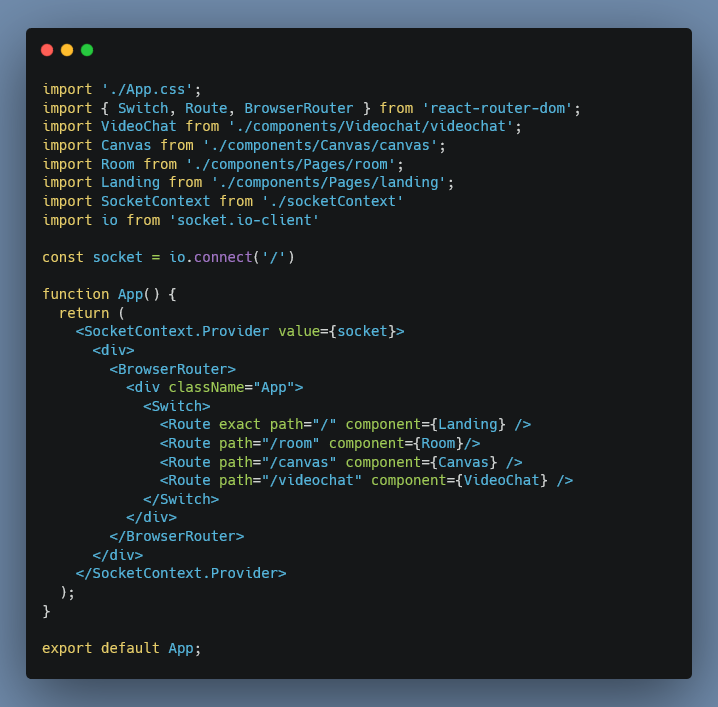
\includegraphics[width=0.8\textwidth]{img/SystemDesign/appJs.png}
    \caption{App.js, source code. Image created using \href{https://carbon.now.sh/}{\textit{Carbon}}.}
\end{figure}

\subsubsection{Landing.js}
When the application is started, the user is routed by the App.js file to this landing page. This page includes an “Enter Room” button, displays credits to the project team developers and displays the “Videsign” logo of which the project is named. When the user clicks the “Enter Room” button, an on-click event is called, which in turn calls a function “enterRoom()”, as seen in Figure 4.5, which reroutes the current page to the “/room” page that presents the user with the Room.js component.
\begin{figure}[H]
    \centering
    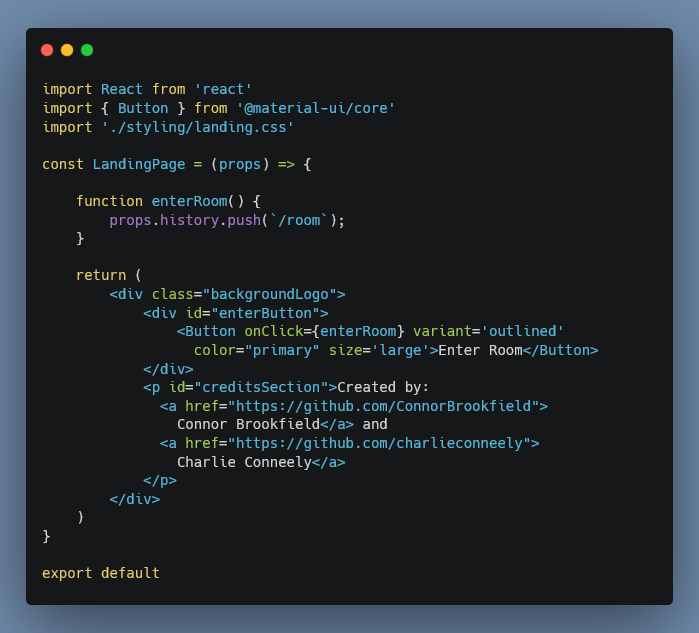
\includegraphics[width=0.8\textwidth]{img/SystemDesign/landingPageJs.png}
    \caption{Landing.js, source code. Image created using \href{https://carbon.now.sh/}{\textit{Carbon}}.}
\end{figure}

\subsubsection{SocketContext.js}
This component creates a React context that is used in the “Room.js” file to assign Socket.IO sockets. React contexts provides an alternate way to pass data through a component tree, instead of using props to manually pass data at every level of the tree. The source code for this class is present in Figure 4.6.
\begin{figure}[H]
    \centering
    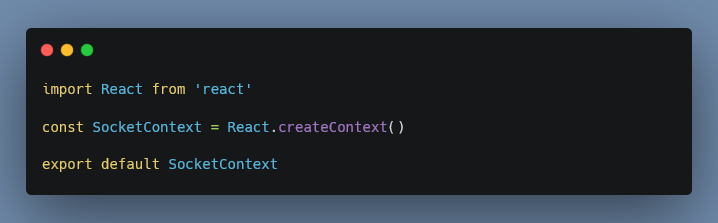
\includegraphics[width=0.8\textwidth]{img/SystemDesign/socketContextJs.png}
    \caption{SocketContext.js, source code. Image created using \href{https://carbon.now.sh/}{\textit{Carbon}}.}
\end{figure}

\subsubsection{Room.js}
Initially upon running this Room component, it imports the “useLocalStorage” component, the “UUID” package, the “Canvas” component, the “VideoChat” component and the “SocketContext” component. It then declares a React hook for the ID of the canvas user and stores it using the “useLocalStorage” component and declares a hook for the “windowWidth” of the canvas component. This ID is then set to a uniquely generated identifier using the UUID packaged installed from the NPM. The width value of the current window is collected and then sets the “windowWidth” hook using that value. In the render/return section of the file, a “SocketContext” component is wrapped around an instance of and passes socket information to the “VideoChat” component. Another “SocketContext” component is used and is wrapped around an instance of the “Canvas” component where the socket information, “userID”, and the “windowWidth” is passed through, as shown by the image in Figure 4.7.
\begin{figure}[H]
    \centering
    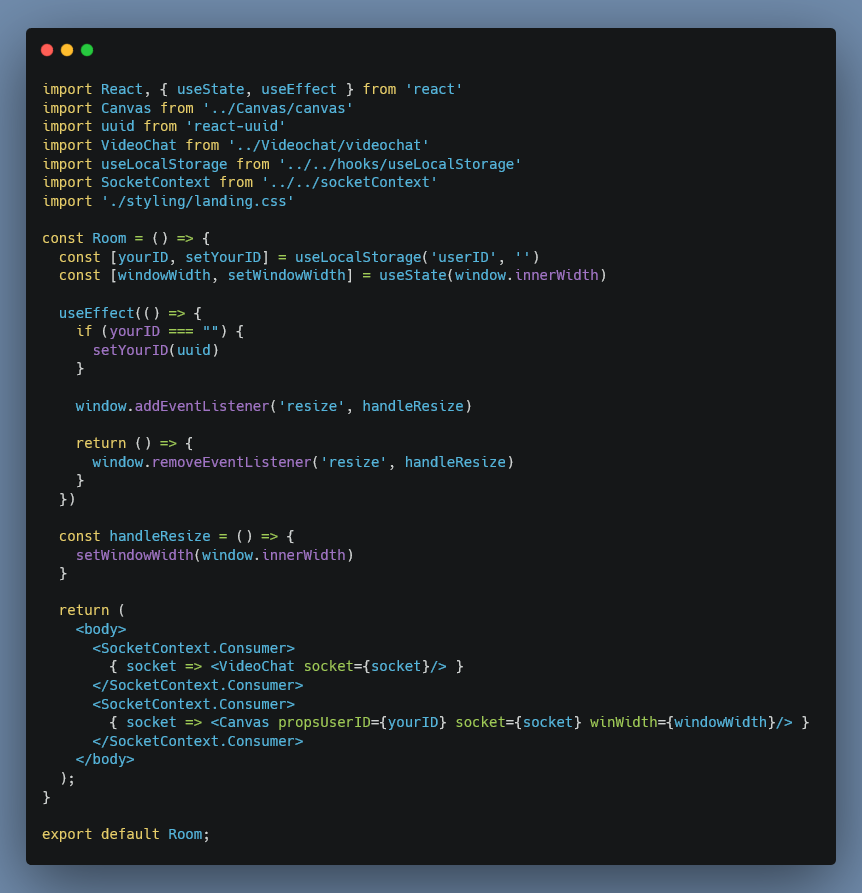
\includegraphics[width=0.8\textwidth]{img/SystemDesign/roomJs.png}
    \caption{Room.js, source code. Image created using \href{https://carbon.now.sh/}{\textit{Carbon}}.}
\end{figure}

\subsection{Video Chat Component}
\subsubsection{videochat.js}
This Video Chat component, is a react component which allows the user to send and receive video and audio streams using peer to peer communication derived from the WebRTC JavaScript API (a native API inbuilt into most modern browsers to allow peer to peer and real-time communication of text, audio, and video). This component in relation to the architecture of the project, is instantiated inside of the Room.js file, or the “room” React component.

For the following paragraphs, all the source code referenced can be viewed below in Figure 4.8. At the start of the Video Chat component, we create React references to document object model (also referred to as the DOM) nodes or in our case React video elements, for rendering the Video/Audio streams later on in the code.

Next, the component creates actions for socket events which are emitted by the socket server (this server is explained in the section 4.1.3). When a successful connection has been made to another candidate (also referred to as a peer), details containing the “success” connection data are printed to the console. When the “offerOrAnswer” socket event has been triggered, a call notification is rendered on the screen of the peer you are calling, thus notifying the user that they are being called. A peer connection then sets a new remote session description containing peer SDP information. The SDP is a protocol that is used in this context to describe media communication data such as negotiation between peers to inform the other of audio codecs, video codecs, network topologies and information about the input devices used. The next socket event labelled “candidate”, passes candidate data into the function, and then creates and adds a new “RTCIceCandidate” using that candidate data, to the “peerConnection” variable. “RTCIceCandidate” is an interface that represents the Internet Connectivity Establishment configuration for the candidate \cite{rtcicecandidate}.

The “peerConnection\_config” constant is then created using a list a publicly free and available “STUN” servers offered by Google. These “STUN” servers allow the user to, transmit data around NAT connections. When you connect to the STUN server, it essentially returns the IP address, port, and connectivity status of a peer, which helps act as an initial gateway which allows you to guide your connection directly to the other peer \cite{stun}. This “peerConnection\_config” is then used to instantiate a new constant RTCPeerConnection object called “peerConnection”, which represents a WebRTC connection between the local machine and the remote peers its connecting to, and features methods to manage and maintain those connections \cite{rtcpeerconnection}.

A constant function named “sendToPeer” is then created. This function takes in a “messageType” and a “payload” variable which are then emitted by this function as a socket event as an event of type “messageType”. This function is used to send the “payload” and “socketID’s” to peers.
\begin{figure}[H]
    \centering
    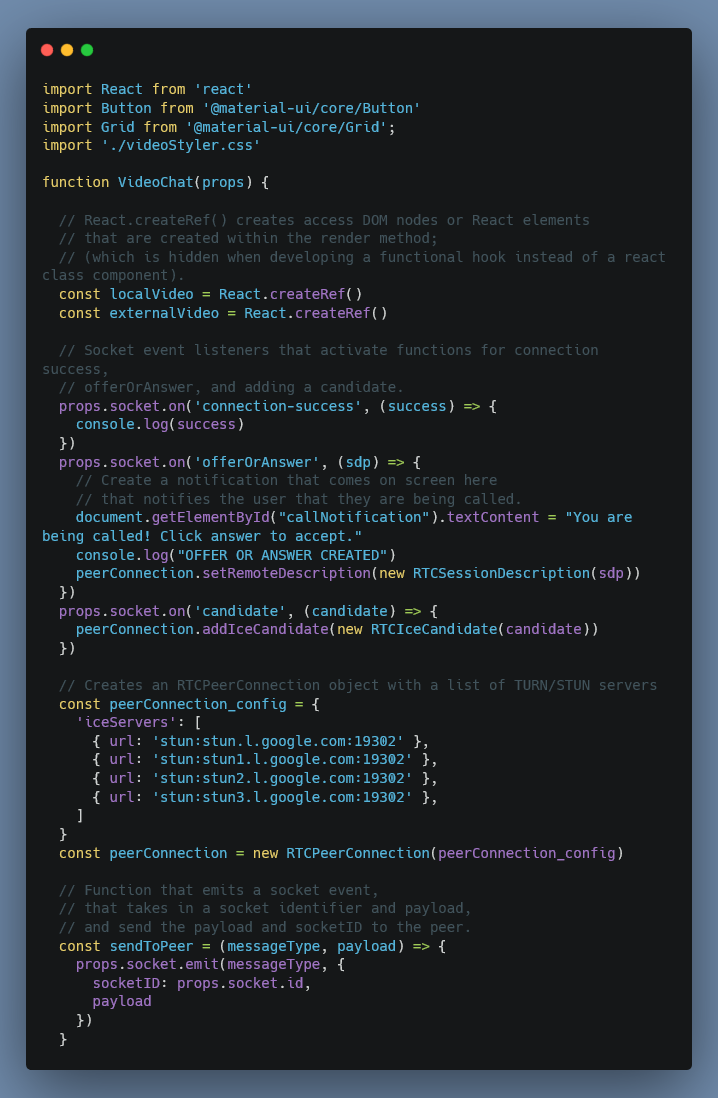
\includegraphics[width=0.8\textwidth]{img/SystemDesign/videoChatJs_1.png}
    \caption{VideoChat.js, source code part 1. Image created using \href{https://carbon.now.sh/}{\textit{Carbon}}.}
\end{figure}

For the following paragraphs, all the source code referenced can be viewed below in Figure 4.9. After defining the “sendToPeer” function, the "peerConnection” object calls an event handler that specifies a function that occurs whenever the local machine’s ICE agent needs to deliver a message to a peer through the signalling server. The function in this case, calls the “sendToPeer” function, passing in the candidate data which was passed through from the even handler. It also logs the candidate data to the console in JSON format. Another event handler is initiated which looks out for connection state changes of the ICE, and logs it to console \cite{rtcpeerconnection}.

The next “peerConnection” event handler called “ontrack” is triggered when a stream has been received from another peer. This calls a function that takes in the event, and assigns the “externalVideo” React reference (as declared at the top of the component function) to the stream of the peer, so that it can display on the other peer’s browser.
Next, a constant function called “createOffer” is created. This function creates a “peerConnection” offer to receive a video stream. If that is successful, then the peerConnection’s local description is set to that SDP, and the SDP is sent to the peer with the “offerOrAnswer” socket event, using the “sendToPeer” function. The next constant function called “createAnswer” is more or less the same as the “createOffer”, with the exception of the peerConnection creating an offer, it creates an answer to receive the incoming video stream. 
\begin{figure}[H]
    \centering
    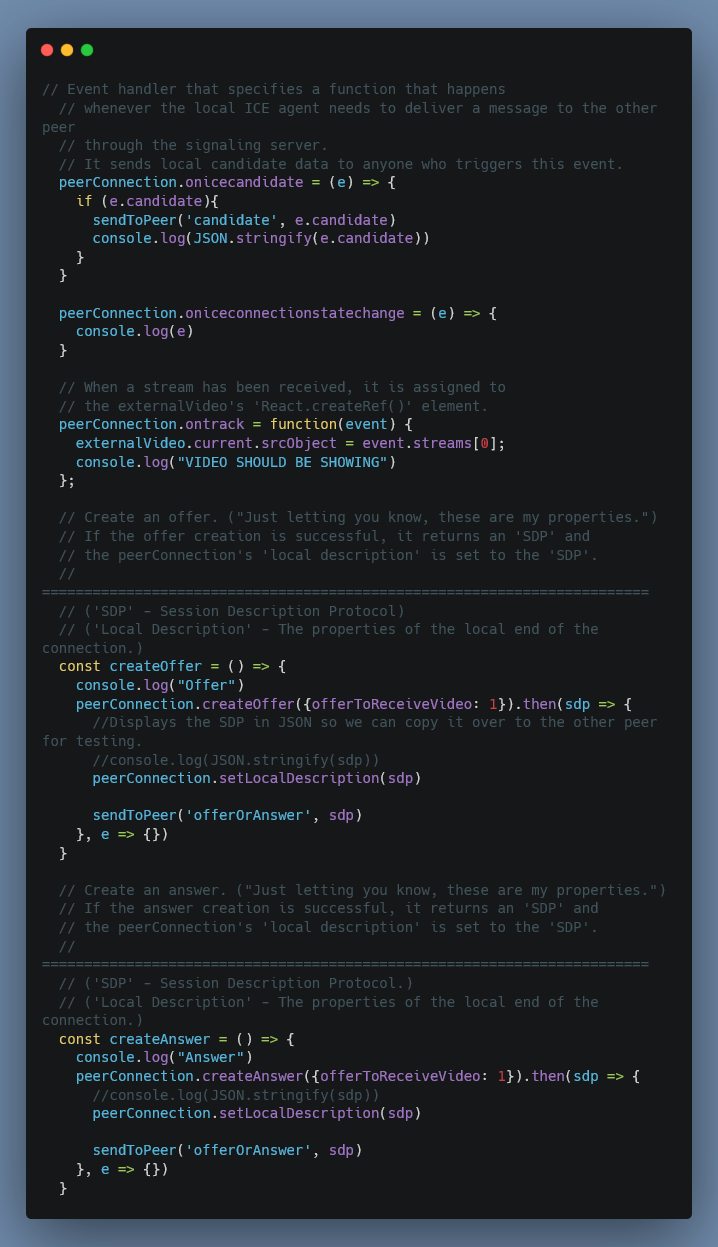
\includegraphics[width=0.8\textwidth]{img/SystemDesign/videoChatJs_2.png}
    \caption{VideoChat.js, source code part 2. Image created using \href{https://carbon.now.sh/}{\textit{Carbon}}.}
\end{figure}

For the following paragraphs, all the source code referenced can be viewed below in Figure 4.10. At the top of this figure, we have a constant function called “mediaSuccess”. This function assigns the local video stream to the React context variable “localVideo” that was created at the top of the component and adds that local video stream to the peerConnection list of streams using the “addStream” method. It also prints out the state of the webcam and microphone permissions to the console. The next constant function “mediaFailure” is a function to outputs a message with the current state of the webcam and microphone permissions to the console.

The navigator tries to grab the user media from the user’s local input media devices in the web browser using promises, depending on whether or not the permissions have been excepted or denied. If the user gives the navigator media permissions for both video and audio, the “mediaSucess” function is called. If the user does not give the browser permissions to use an audio and video device, the “mediaFailure” function is called.

The return section of this code renders HTML on the screen. In this instance, a “<Grid>” element, taken from the “Material-UI” package installed via NPM, creates a grid with a container spacing of  2, which displays both the local video stream as agrid item, and the external video stream from the connected peer as a grid item, by referencing the React context variables defined at the top of the JavaScript component. Another grid item is created to display the call notification to notify the user when they are being called. The last two items in the grid container are the call and answer buttons. These buttons utilise the buttons from the “Material-UI” package, and both feature “onClick” events. The “Call” button calls the “createOffer” function when the “onClick” event is triggered, while the “Answer” button calls the “createAnswer” function when the “onClick” event is activated.

\begin{figure}[H]
    \centering
    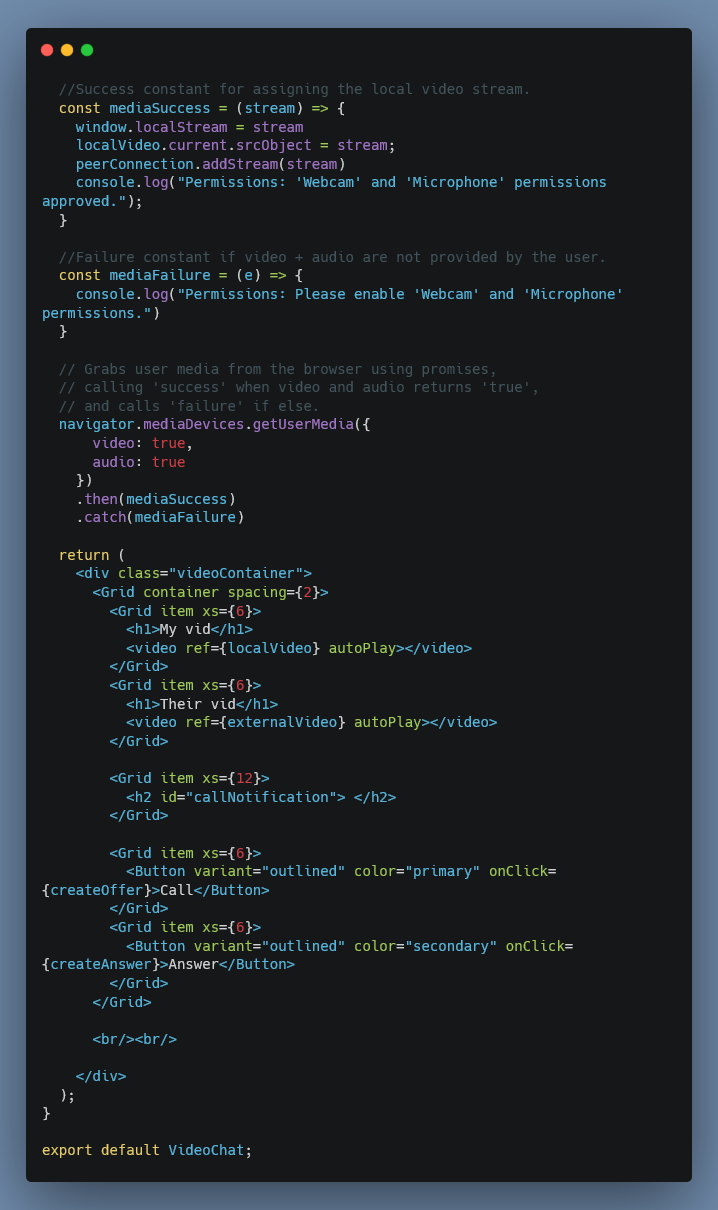
\includegraphics[width=0.8\textwidth]{img/SystemDesign/videoChatJs_3.png}
    \caption{VideoChat.js, source code part 3. Image created using \href{https://carbon.now.sh/}{\textit{Carbon}}.}
\end{figure}
\subsection{Server Back-end}
This express server was created to serve as an event listener for socket events for the Video Chat and Canvas components of this project. When the user of this application compiles and runs the build of this project, the server also renders the application.
\subsubsection{Server.js}
For the following paragraphs, all the source code referenced can be viewed below in Figure 4.11. 
This express server was created to serve as an event listener for socket events for the Video Chat and Canvas components of this project. When the user of this application compiles and runs the build of this project, the server also renders the application.
At the top of the Server.js file, all the constants required for the server’s operation are declared. These constants are the barebones requirements to turn the Server.js file into an express application and then a web server for socket connections. After the declaration of the fundamental constants required, the server renders a static version of the built React application. It then gets the root directory of the built application and redirects the user to the “index.html” file within the build folder. The server then creates a map of all the peer connections to Socket.IO sockets.

The next function of the server is to serve some defined Socket.IO server-side event listeners. The first event listener created called “connection”, listens to when a peer connection has been established to the server and passes in its socket. The function outputs the ID of the socket of the connected peer, it emits a “connection-success” event while passing through its socket ID for application side processing. The “peerConnections” map adds another peer setting the socket ID as the key and the socket as the value.

Within this “connection” event is another event listener for the socket that has just connected. This event listener called “join-room” takes in a “roomID” and a “userID” and listens to the socket and waits for it to emit the event. This event listener tells the connected socket to join the “roomID” and emits a “user-connected” event with the peer’s “userID” to all sockets connected to that “roomID”. The socket also listens for when the socket triggers the “disconnect” event, and emits a “user-disconnected” event along with the peer’s “userID” to all peers with the same “roomID”.

\begin{figure}[H]
    \centering
    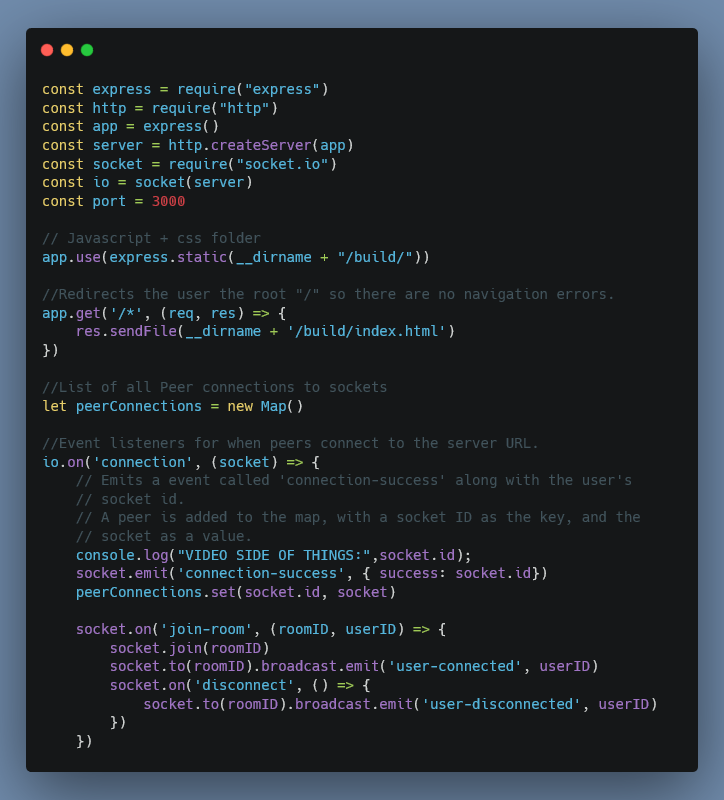
\includegraphics[width=0.8\textwidth]{img/SystemDesign/serverJs_1.png}
    \caption{Server.js, source code part 1. Image created using \href{https://carbon.now.sh/}{\textit{Carbon}}.}
\end{figure}
For the following paragraphs, all the source code referenced can be viewed below in Figure 4.12. The next event listener for sockets inside of the main “connection” event is the “offerOrAnswer” event which takes in “data”, which is passed in as the SDP by the client side of the application. This event iterates through all of the entries inside of the “peerConnections” map, and checks if the local loop variable instance “socketID” is compared with the “data”s socket ID. If the two IDs differ, the server emits a “offerOrAnswer” event with the payload data, and outputs the local socket ID and the payload from the “data” are outputted to the console.
After this event listener, an almost identical event listener called “candidate” is present, taking in the same “data” as the previous. The difference between this event listener and the previous, is that it emits a “candidate” event if the loops socket ID and the passed through socket ID do not match.

The server then listens for a “disconnect” event listener, emits an event called “your id” with the current socket’s ID, and then listens for the “send canvas state” and a “take control” event listeners. The “disconnect” event is triggered when a peer disconnects from the server, which then removes the disconnected peer’s socket ID from the map of peer connections. The “send canvas state” takes in a “body” variable and emits a “canvasState” event with the passed through variable “body”. The “take control” event takes in a “userID” variable and emits a “control switch” event with the “userID” variable passed through with it. 

The final line of code shown in Figure 4.12, allows the server to listen to the predefined port which was declared as a constant with an integer value of “3000” at the top of the Server.js file, and outputs the port the server is listening to in the console.

\begin{figure}[H]
    \centering
    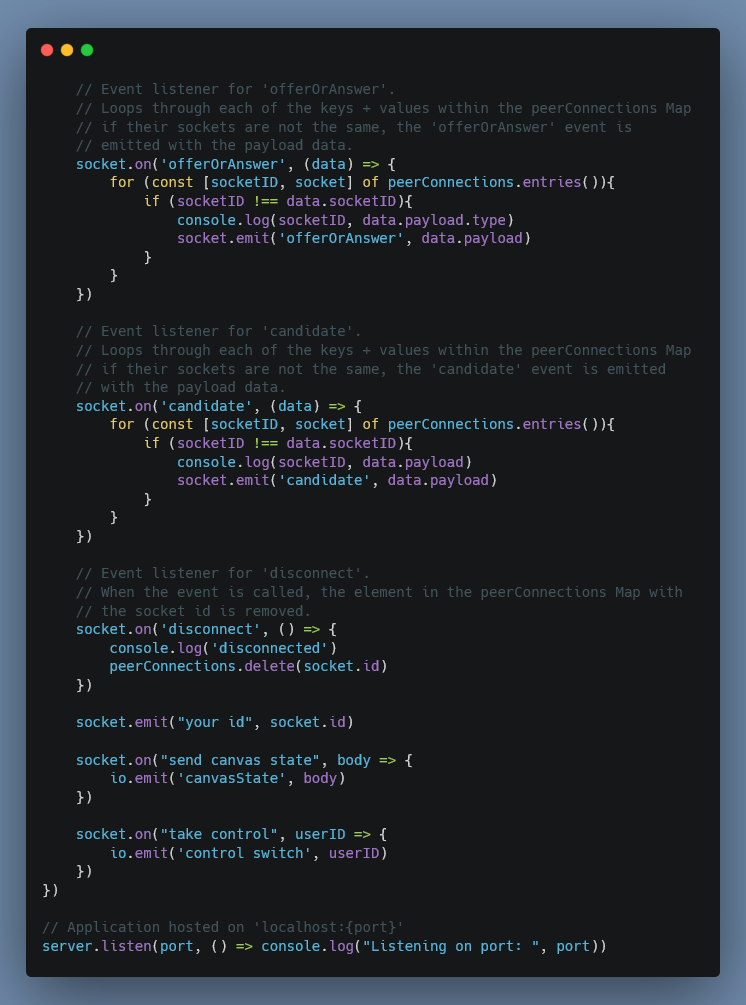
\includegraphics[width=0.8\textwidth]{img/SystemDesign/serverJs_2.png}
    \caption{Server.js, source code part 2. Image created using \href{https://carbon.now.sh/}{\textit{Carbon}}.}
\end{figure}
\subsection{Canvas component}
\label{canvas-component}
\begin{figure}[H]
    \centering
    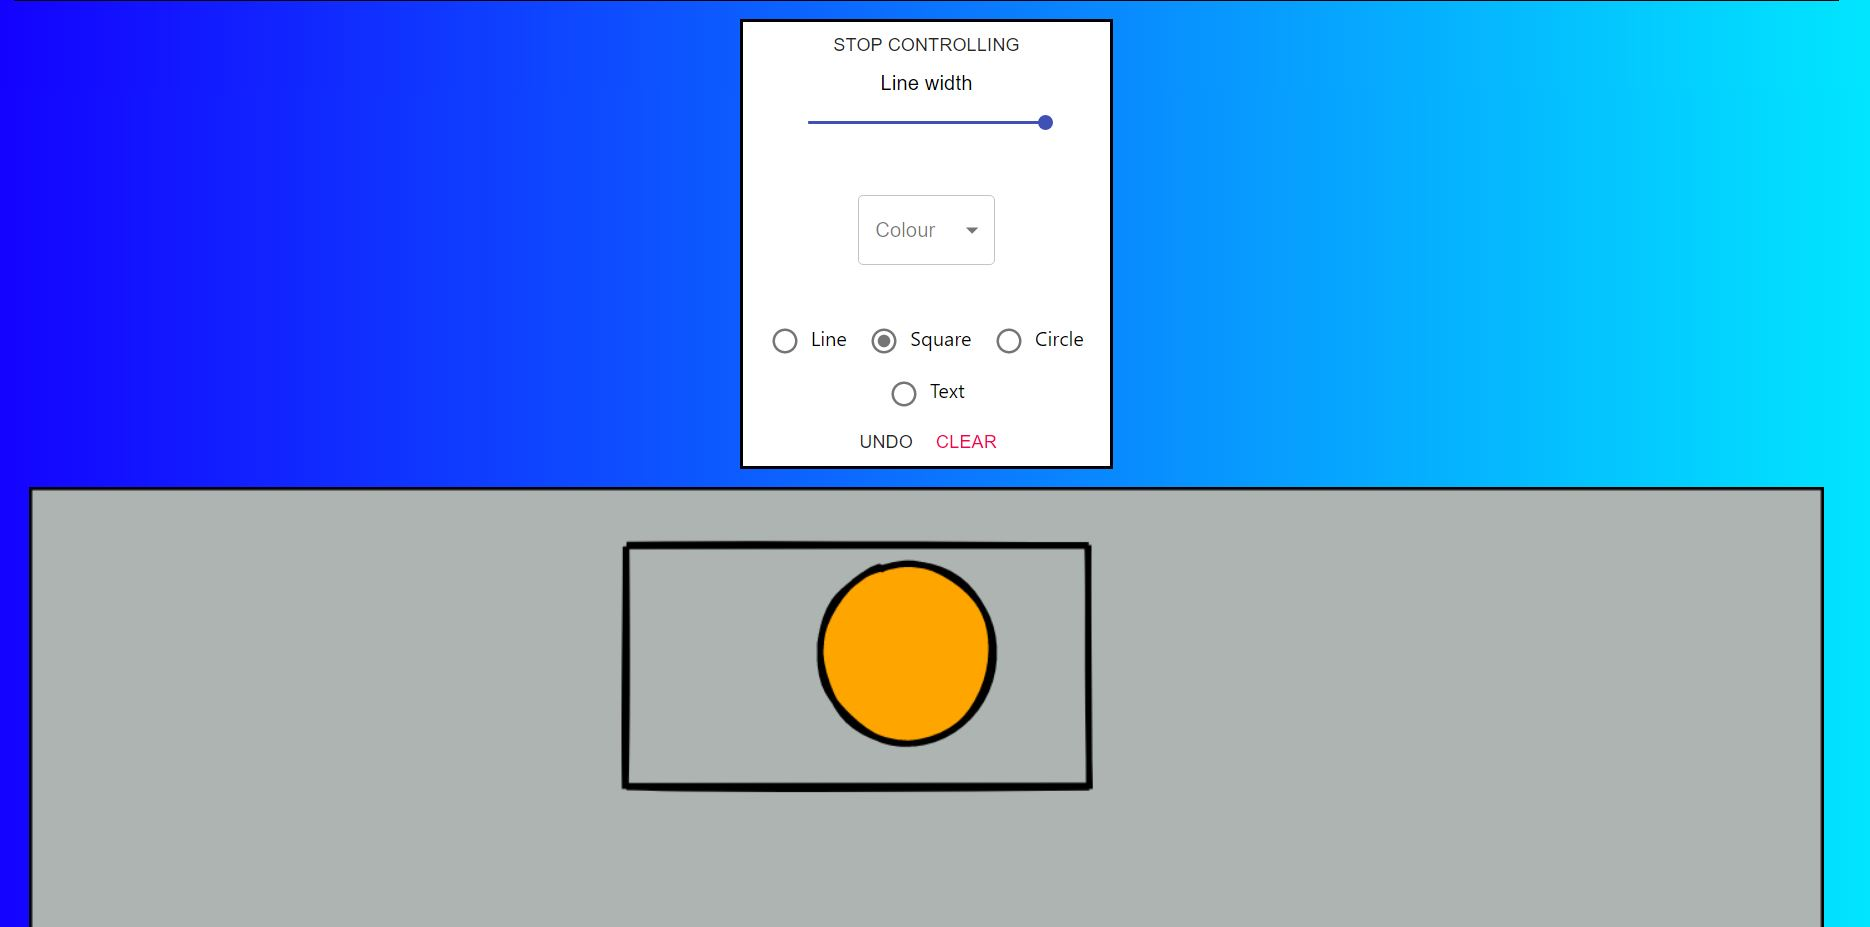
\includegraphics[scale=0.4]{img/SystemDesign/Canvas/canvas-screenshot.JPG}
    \caption{Canvas/Whiteboard Section of the GUI.}
    \label{canvas-screenshot}
\end{figure}

The entire canvas section of the application comprises a root component called Canvas which nests all others such as the Toolbar component and the HTML canvas element inside the Drawing Board component. 

\begin{figure}[H]
    \centering
    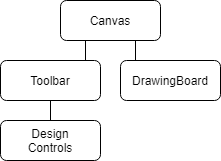
\includegraphics[scale=0.8]{img/SystemDesign/Canvas/canvas-components.png}
    \caption{Canvas Component Tree.}
\end{figure}

\subsubsection{canvas.js}
The Canvas component nests the Drawing Board and the Toolbar components which handle the drawing of shapes and text objects on the canvas.  
Here, we store all of our state variables. These include the elements which are rendered on the canvas and their design characteristics such as line width and colour. We stored all local variables using React Hooks useState or useLocalStorage. 

\begin{minted}{javascript}
// [variable, set function] = useState(default value)
const [isDrawing, setIsDrawing] = useState(false)
const [shape, setShape] = useState("Line")
const [colour, setColour] = useState("") 
const [lineWidth, setLineWidth] = useState(1)
const [inControl, setControl] = useState(false)
const [textSize, setTextSize] = useState(20)
// array of shape objects stored in the browsers local storage
const [elements, setElements] = useLocalStorage("elements", [])
\end{minted}

The Canvas component acts as a point of communication to the Socket.IO functionality on the back end. We defined functions to listen for emitting messages coming through the socket. For example, we define a method called switchControl that will emit the message “take control” through the socket with our unique ID attached. 

\begin{minted}{javascript}
// called from toolBar component
const switchControl = () => {   
    // props.propsUserID = unique ID in parent component 
    props.socket.emit("take control", props.propsUserID)
}
\end{minted}

The Socket.IO back end will, upon receiving this message, emit to all peers the message “control switch”, with this ID attached. We then define a socket.on method that listens for the incoming emit message “control switch”. This method will check if the attached ID is the same as our local ID in the Room parent component. If it is, we set our state variable inControl to be true, if it is not, we set inControl to be false. 

\begin{minted}{javascript}
props.socket.on("control switch", id => {   
    if (id === props.propsUserID) {
        setControl(true);
    } else {
        setControl(false);
    }
})
\end{minted}

Similarly, when we send the canvas state (\textit{elements} array containing the shape objects) across peers, we emit the message "send canvas state". 

\begin{minted}{javascript}
// Called from inside the Drawing Board component.
// If we are not in control - this method will not be called. 
const sendCanvas = (cState) => {
    props.socket.emit("send canvas state", cState);
}
\end{minted}

When the socket receives this message on the back end, it will emit the message "canvasState" to all peers with this array attached. Inside our Canvas component, we have a function that will listen for this message, check if we are not in control (if inControl is false), and update the elements array accordingly. 

\begin{minted}{javascript}
props.socket.on("canvasState", cState => {
    // If we are in control - we emitted the message ourselves
    // and there is no need to update our state. 
    // If not in control - synchronise our state with that of the
    // peer that is. 
    if (!inControl) setElements(cState.body);
})
\end{minted}

\subsubsection{drawingBoard.js}

The DrawingBoard component is essentially the whiteboard of our application. It performs the following tasks:
\begin{enumerate}
    \item \textbf{Create and display the HTML canvas element with conditional interactivity.} \newline 
    The canvas element is interactive because we have attached onMouseDown, onMouseMove, and onMouseUp event handlers that capture the coordinates of the pointer and pass that data into functions. However, we want the canvas to be disabled when we are not in control. To accomplish this, we defined our canvas element using a conditional ternary operator. 
    \begin{minted}{javascript}
// props.propsInControl = inControl variable in parent component Canvas 
// if in control - create a canvas element with mouse event handlers
const canvasElement = props.propsInControl ?
    \end{minted}
    \begin{minted}{html}
<canvas id="canvas"
    width={canvasWidth}
    height={canvasHeight}
    onMouseDown={handleMouseDown(e)}
    onMouseMove={handleMouseMove(e)}
    onMouseUp={handleMouseUp}>
</canvas>
<!-- else - return non-interactive canvas -->
:
<canvas id="canvas"
    width={canvasWidth}
    height={canvasHeight}>
</canvas> 
    \end{minted}

    We then insert this canvas element into our HTML. 

    \begin{minted}{html}
<div>
    {canvasElement}
</div>
    \end{minted}

    \item \textbf{Create and add shape objects to the elements array using the event-handlers from the canvas element.} 
    
    \textbf{onMouseDown} \newline 
    The goal here is to render a shape on the canvas immediately when/where the user clicks on the canvas. \newline When we left-click on the canvas element of the document, the onMouseDown event will trigger a function called handleMouseDown, passing in the \textit{x} and \textit{y} coordinates of the pointer. First, this function will offset the outer edges of the canvas, so that the x and y coordinates match the positioning of the pointer exactly. Next, it will check if the \textit{shape} variable in the parent components state is equal to "Text". If it is, we will create a text element and add it to the elements array with a property called \textit{type} set to "text". If the value in \textit{shape} is set to anything else, we will pass this value, along with the coordinates and a few other parameters to the shapeGenerator function, which will return a shape object to be appended to the elements array. 
    
    \textbf{onMouseMove} \newline
    While we hold the mouse click down, we want the shape on the canvas to re-render constantly under the position of the pointer. \newline 
    When we move our mouse, we trigger the handleMouseMove function. However, we only want this function to execute fully when the user is holding down the left-click. Otherwise, the canvas would constantly render shapes as the user moves the mouse. \newline
    As a solution, we created a state variable \textit{isDrawing}. On the onMouseDown event, this variable will be set to true. On the onMouseUp event (when the user releases the left-click), it will be set to false. Using this variable, we can now determine when the user is intending to draw. \newline 
    At the beginning of the handleMouseMove method, we implemented a guard clause to exit the function when the \textit{isDrawing} variable is false. 
    \begin{minted}{javascript}
const handleMouseMove = (event) => {
    if (!isDrawing) return;
    ...
}
    \end{minted}
    Next in the handleMouseMove function, we will retrieve the \textit{x} and \textit{y} coordinates of the pointer as before along with the coordinates of the last shape element on the \textit{elements} array. Using these two sets of coordinates, we can create a new shape with the shapeGenerator function. Finally, we will overwrite the last item on the \textit{elements} array with our new shape. 
    
    \begin{minted}{javascript}
const handleMouseMove = (event) => {
    if (!isDrawing) return;
    var {pageX, pageY} = event;
    // Account for offset
    var xPos = pageX - canvas.offsetLeft;
    var yPos = pageY - canvas.offsetTop;
    // Retrieve x,y coords of last item on elements array
    var index = elements.length - 1;
    var {x1, y1} = elements[index];
    // create a new shape 
    var currentElement = shapeGenerator(shape, colour,
        x1, y1, xPos, yPos, lineWidth);
    const elementsCopy = [...elements];
    // replace last item with new shape 
    elementsCopy[index] = currentElement;
    // overwrite elements array on state 
    setElements(elementsCopy);
}
    \end{minted}
    
    \textbf{onMouseUp} \newline 
    The onMouseUp event occurs when we release the left-click on the mouse and it will trigger the handleMouseUp method. This method will first set the \textit{isDrawing} variable to false to show that we are no longer drawing. \newline
    Next, it will check if the \textit{inControl} variable is set to true. If it is, we will emit the "send canvas state" message as before, attaching the elements array. 
    \begin{minted}{javascript}
const handleMouseUp = () => {
    setIsDrawing(false);
    if (!InControl) return;
    // if in control - send updated elements array across socket
    const canvasObject = {
        body: elements,
        id: id
    }
    sendCanvas(canvasObject);
}
    \end{minted}
    
    \item \textbf{Render all shapes in the elements array on the canvas.} \newline
    At this stage, we have outlined how we can create shapes using mouse events and save them to an array. However, we still need to draw all of these shapes on the canvas, and we need this to happen every time the \textit{elements} array changes. \newline
    To accomplish this, we implemented the \textit{useLayoutEffect} React hook. The \textit{useLayoutEffect} hook works the same as \textit{useEffect}, which will execute when the page loads, and when a particular item changes. We can specify this item by passing it into an array at the end of the hook declaration. We chose \textit{useLayoutEffect} specifically because it was designed to fire synchronously with the resulting DOM update. This characteristic makes it an ideal choice for this application, as we do not want there to be any visual inconsistencies for the end-user. \newline
    At the end of our \textit{useLayoutEffect}, we passed the \textit{elements} array and the window size: \textit{window.width}. We passed in \textit{window.width} because we want our shapes to redraw themselves to scale when the window changes size. Now, each time the window is resized or the \textit{elements} array changes, \textit{useLayoutEffect} will execute. \newline
    First, inside \textit{useLayoutEffect}, we define the canvas and context variables and connect our canvas to the Rough JS library as illustrated in Section \ref{canvasSection}. We then need to clear the canvas so that we are not redrawing the same elements on top of each other repeatedly. 
    
    \begin{minted}{javascript}
useLayoutEffect(() => {
    var canvas = document.getElementById("canvas");
    var context = canvas.getContext('2d');
    // connect our canvas to rough js 
    var rc = rough.canvas(canvas)
    
    // clear context
    context.clearRect(0, 0, canvas.width, canvas.height);
    // redefine styling features
    context.lineWidth = 5;
    context.strokeStyle="black";
    context.strokeRect(0, 0, canvas.width, canvas.height);
    
    ...
    
}, [elements, window.width])  
    \end{minted}
    
    Next, we will loop through the elements array and check first if each element has a property called "type". If it does, this means that this element is a text object. In this case, we will use methods that the context exposes to render this text on the canvas. \newline
    If the "type" property is not present, we will call the \textit{draw} function that Rough JS provides, passing in our shape object. 
    
    \begin{minted}{javascript}
useLayoutEffect(() => {
    
    ...
    
    elements.forEach(e => {
        // check if item is a text element
        if (e.hasOwnProperty('type')) {
            context.font = e.size + 'px serif';
            // draw on canvas - (value, x, y)
            context.fillText(e.val, e.xco, e.yco);
            return;
        }
        rc.draw(e.roughElement)
    });
}, [elements, window.width])    
    \end{minted}
    
\end{enumerate}

\subsubsection{toolbar.js}
The Toolbar component provides the end-user with buttons to take control of the canvas, undo the last element, and clear the entire canvas. It also provides radio buttons so that the user can select what type of graphic they would like to draw: line, square, circle, or text. The DesignControls component from shapeDesignControls.js that handles the colour and line width controls is also nested inside Toolbar.

\begin{figure}[H]
    \centering
    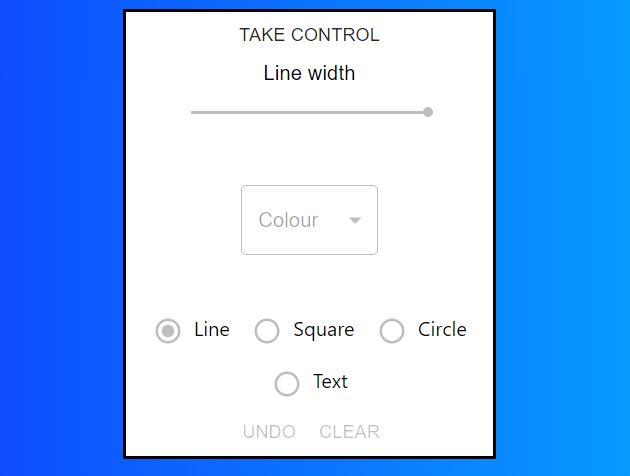
\includegraphics[scale=0.6]{img/SystemDesign/Canvas/toolbar-screenshot.JPG}
    \caption{The Toolbar Component.}
\end{figure}

The "Take Control" button calls a method that will change the boolean state variable \textit{inControl} to !\textit{inControl}. If the user was not in control before the button click, we will call the function to handle the appropriate Socket.IO communication.  
\begin{minted}{javascript}
const switchControl = (e) => {
    e.preventDefault();
    if (inControl) {
      setControl(false)
      return
    }
    setControl(true)
    // socket.io function
    switchControl() 
}
\end{minted}

The radio buttons for the shape will all simply set a shape variable on the state to their assigned value. The system will eventually pass the shape variable into the \textit{shapeGenerator} function, which will return a shape object to be added to the elements array and rendered on the canvas.

The button titled Undo will call a function of the same name. The undo function will remove the last element from the \textit{elements} array and send this updated array through the socket connection. 

\begin{minted}{javascript}
const undo = (e) => {
    e.preventDefault()
    if (!inControl) return;
    // retrieve index of last item
    var index = elements.length - 1
    const copy = [...elements]
    // Remove last element from state
    copy.splice(index, 1)
    // overwrite state array of elements
    setElements(copy)
    // send updated array across peers 
    sendCanvasAcrossPeers(copy)
}
\end{minted}

Similarly, the clear button will call a method to empty the \textit{elements} array entirely, and send this empty array through the socket connection.

\begin{minted}{javascript}
const clearCanvas = (e) => {
    e.preventDefault()
    if (!inControl) return;
    // empty canvas array of elements
    setElements([])
    // send canvas state to peers
    sendCanvasAcrossPeers([])
}
\end{minted}

One important feature of the Toolbar is that when the user is not in control, all inputs are disabled. We accomplish this by defining a variable called \textit{isDisabled} which is assigned the value of !\textit{inControl}. So when the user is not in control of the canvas, \textit{isDisabled} will be true. Inside the HTML, all tags for the buttons and radio buttons have their disabled attribute set to the value assigned to \textit{isDisabled}. 

\begin{minted}{javascript}
const isDisabled = !inControl;
\end{minted}
\begin{minted}{html}
<!-- inside the HTML --> 
<Button onClick={undo(e)} disabled={isDisabled}>Undo</Button>
\end{minted}

\begin{figure}[H]
    \centering
    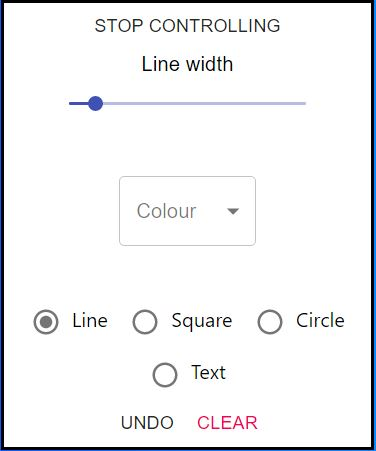
\includegraphics[scale=0.6]{img/SystemDesign/Canvas/inControlToolbar.JPG}
    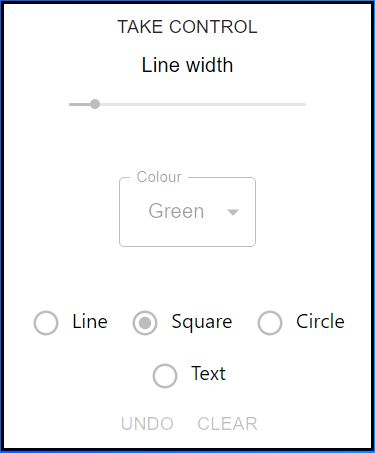
\includegraphics[scale=0.6]{img/SystemDesign/Canvas/notInControlToolbar.JPG}
    \caption{Enabled and Disabled Toolbar}
\end{figure}

\subsubsection{shapeDesignControls.js}
The DesignControls component provides a slider to control the line width, and a drop-down list to select the colour. Eventually, we will pass these parameters into the \textit{shapeGenerator} function.  

To provide these UI components, we implemented the following items from the Material UI library. 

\begin{minted}{javascript}
import { FormControl, InputLabel, Select, MenuItem, 
    Typography, Slider } from '@material-ui/core'
\end{minted}

These control options were separated from the Toolbar component to improve code readability. 

\subsubsection{shapeGenerator.js}
The shapeGenerator function utilises the Rough JS generator as outlined in Section \ref{canvasSection}. The DrawingBoard component will pass, as arguments into the function parameters, the shape coordinates, combined with the shape type (“Circle”, “Line”, etc.), colour and line-width values from the Toolbar.  

Inside the function, we first need to determine what shape is being requested. To accomplish this, we will use an \textit{if/else if} statement to check the value of the \textit{shape} parameter. If the value of \textit{shape} is “Square”, then we will use the remaining parameters to create a shape object as follows.

\begin{minted}{javascript}
function shapeGenerator(shape, colour, x1, y1, x2, y2, lineWidth) {
    // define variable
    var roughElement;
    if (shape === "Square") {
        // create a rectangle using 
        // generator.rectangle(x, y, width, height)
        roughElement = generator.rectangle(x1, y1, x2 - x1, y2 - y1, {
            fill:colour,
            fillStyle:'solid',
            strokeWidth: lineWidth
        })
    }
    
    ...
    
}
\end{minted}

If the value of \textit{shape} is not "Square", we will check if it is "Circle". If it is, we will create a circle shape using the remaining parameters as follows.

\begin{minted}{javascript}
...

else if (shape === "Circle") {
    // set centre points to midpoint between 
    // original & current mouse location
    var xCentre = x2 - ((x2-x1)/2)
    var yCentre = y2 - ((y2-y1)/2)
    // create a circle using generator.circle(x, y, diameter)
    roughElement = generator.circle(xCentre, yCentre, (x2 - x1)*2, {
        fill:colour,
        fillStyle:'solid',
        strokeWidth: lineWidth
    })
}

...
\end{minted}

Finally, if neither conditions are satisfied, we will incur that the shape is a "Line", and create a line shape object as follows: 

\begin{minted}{javascript}
...

else {
    roughElement = generator.line(x1, y1, x2, y2, {
        strokeWidth: lineWidth
    })
}
return {x1, y1, x2, y2, roughElement};
\end{minted}

As illustrated above, at the end of the function, we pass the \textit{roughElement} variable back to the DrawingBoard component along with the coordinates to be saved in the \textit{elements} array on state. Later, we will pass the object stored in the \textit{roughElement} variable into the \textit{draw} method. As the Rough JS library created this object, the \textit{draw} function will handle it properly and render it on the DOM.  

\section{Design Principles}
For this project, our project team found it crucial to implement good design principles at the initial planning phase. Our project team settled on utilising the SOLID principles. These principles (as described in section 3.1.4) were used intensively throughout this project as intended. The first principle “S” in SOLID, which stands for the “Single Responsibility Principle”. This principle ensures that any class or code that is written has a single function, which in our project was the breaking up of features into different React components such as the Canvas has the single responsibility of the execution of only canvas related functions, and the Video Chat component has the single responsibility to only do video/chat related functions.

The next principle “O” in SOLID, is the “Open Close Principle”. The principle enforces the idea that different modules should designed so that they shall never be changed but can be extended and an extension of that functionality can be modified. In our project, each function and class has been designed to allow the functionality to be implemented and overwritten, but using JavaScript and React make this a little more difficult to practically implement in comparison to an object oriented programming language such a Java which makes the process of extending classes much more intuitive.

Much like the previous principle, “L” in SOLID called the “Liskov Substitution Principle”, is better suited to object oriented programming languages of which JavaScript is not fully. This principle informs us that if you use a function or make references to base classes, that the function or reference should be able to use derived objects without knowing that it is  accessing the base class. This means we could substitute a superclass object reference with an object of any of its subclasses. In our project, we did not use any object derivatives, but our project team kept this principle in mind when designing the application.

The “Interface Segregation Principle” (the “I” in SOLID) infers that interfaces should not be forcefully depended on if they are not being used by a client. This means that a client should use separate interfaces instead of depending too heavily on a single interface with multiple functions that might break another part of an application when one of those functions have changed.

The last of the SOLID principles, “D”, is called the “Dependency Inversion Principle”. This principle states that high-level and low-level modules should not depend on each other but should instead depend on abstractions so that these modules can be highly decoupled \cite{singh2015effect}.

Our project team have coded components and classes in a way that allows these principles to work once more object-oriented features become more prevalent within JavaScript.

\chapter{System Evaluation}

\section{Testing}
\subsection{Acceptance Tests}
We performed acceptance tests by running the application locally on two separate windows, one of which needs to be incognito, each sharing half of the monitor. For brevity, we will refer to these windows as Peer A and Peer B. Through our acceptance tests, we confirmed the following:   

\begin{itemize}
    \item The application starts on the Landing component and the "Enter Room" button should bring us directly to the Room component. 
    \item When Peer A and Peer B have both reached the Room component, the two should be connected as peers through Socket.IO. 
    \item When Peer A clicks the call button, Peer B should be notified of this. When Peer B clicks accept, the media stream of both peers will be communicated and displayed properly. 
    \item The audio and visual data communicated between peers through WebRTC is clear and that the design of the applications GUI supports this.
    \item The graphics being drawn on the canvas render on the DOM of each peer fast enough to give the illusion that they are rendering synchronously.       
    \item When Peer A hits the take control button, Peer B should lose control immediately and vice versa. 
    \item All UI components on the toolbar should work properly.
\end{itemize}

\begin{figure}[H]
    \centering
    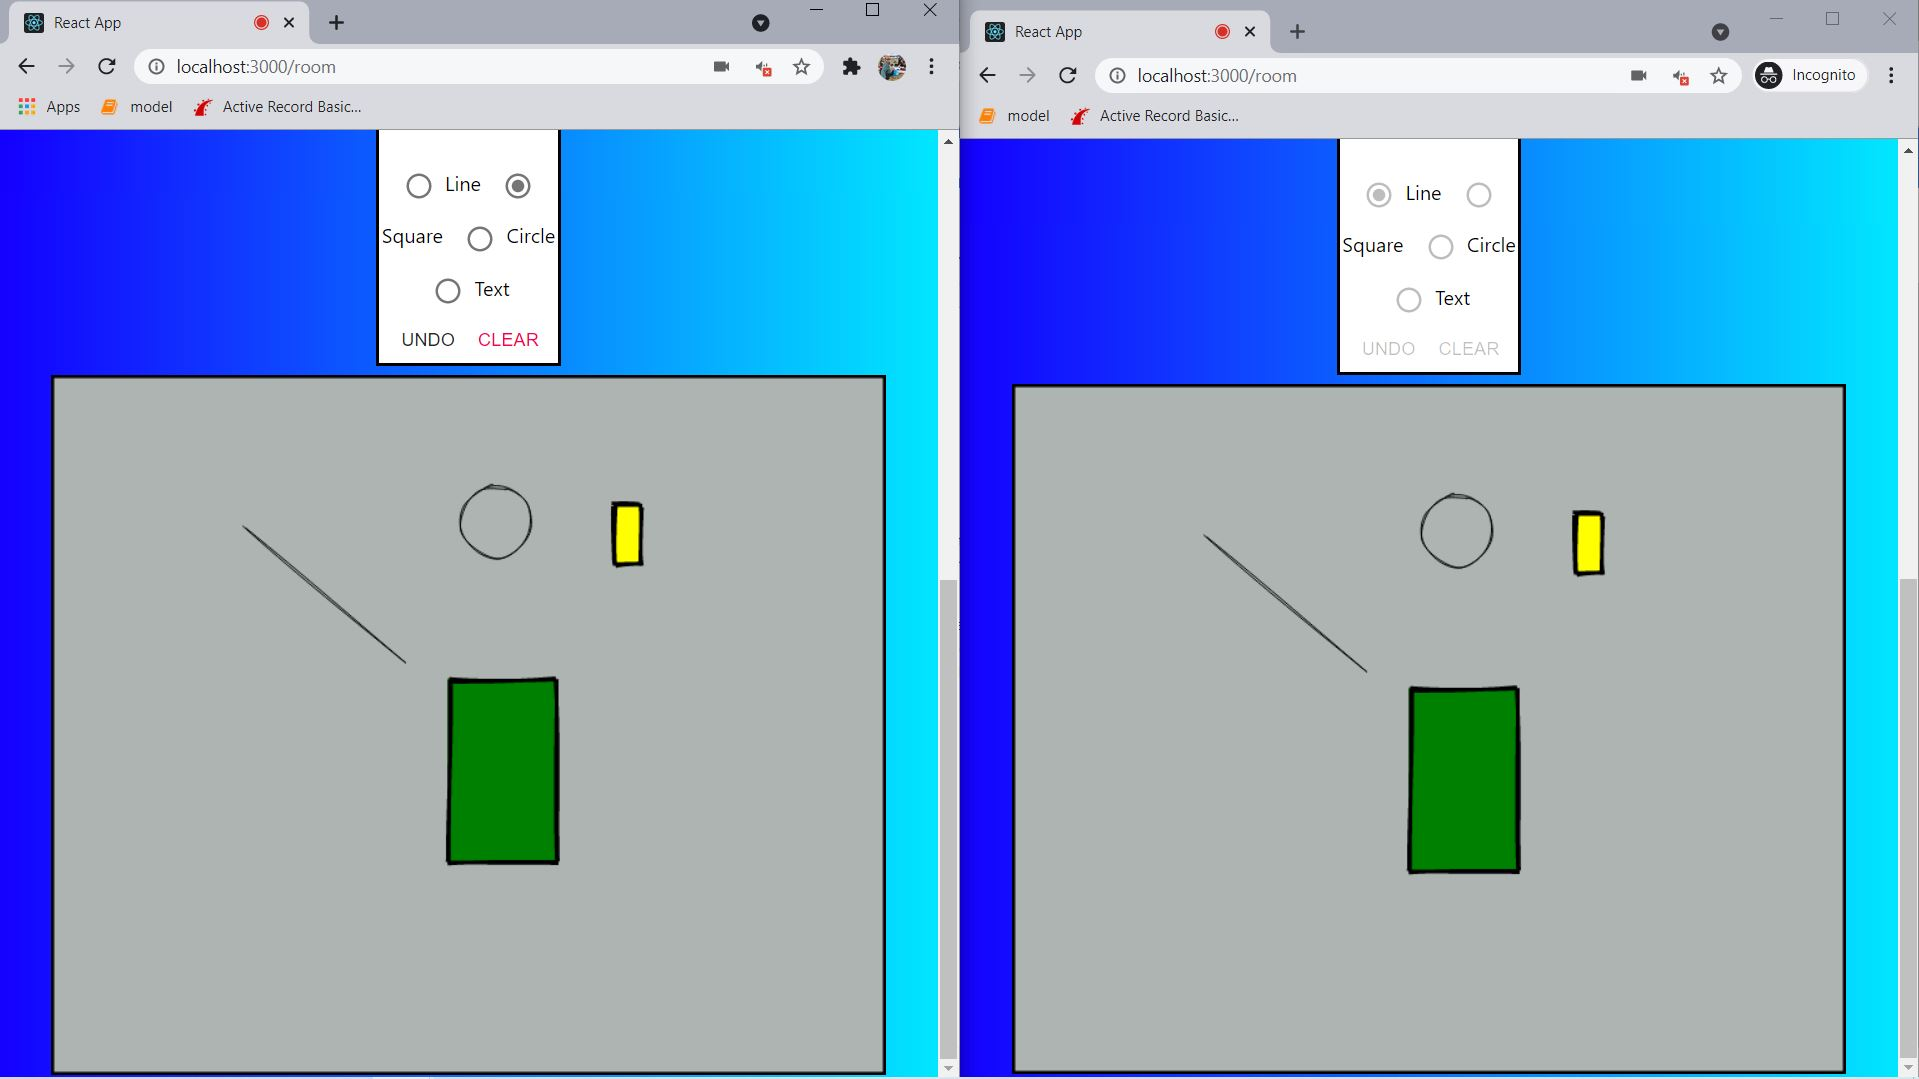
\includegraphics[scale=0.3]{img/Evaluation/canvas-testing.JPG}
    \caption{Canvas Acceptance Tests}
    \label{canvas-acceptance}
\end{figure}

\subsection{Selenium}
\label{selenium}
For this project, our project team decided to use Selenium for testing UI components within the application. Our project team installed a Selenium plugin for Firefox and Chrome, called Selenium IDE. This plugin is an integrated development environment for Selenium, that allows tests to be recorded within the browser through user clicks and navigation, and it allows for tests to be edited manually and debugged. 

This plugin was effective and well suited to test the user navigation from the root page to the room page. It also allowed for us to check the functionality of the application by replicating slider movement within the tool section of the canvas, as well as the ability to draw within the canvas. Upon reflection, Selenium was an easy to use tool that was beneficial to our project team to replicate user functionality through continuous integration testing for major code changes and versions.

\section{Outcome}
In the beginning, we aimed to create a peer-to-peer web conferencing application using WebRTC, React, and Socket.IO that would enable peers to communicate through audial and visual means. We also intended for the application to supply an interactive whiteboard that both participants could use to aid clear communication. In the end, we created an application that utilises these technologies effectively and that provides the service as outlined above. However, early in our planning stage we outlined several features that the application should provide beyond the basic functionality. 

We wanted the whiteboard element of the application to provide the end-user with enough tools so that they can comfortably illustrate their ideas onto the canvas, without having to make sacrifices. We achieved this as we developed a toolbar which enabled the user to draw lines, circles, rectangles, and plain text. Through a combination of these shapes, the end user should be able to illustrate a standard business-related diagram. However, there are still many elements that would improve the system greatly that unfortunately, due to time constraints, went unimplemented. These include arrows, triangles, or icons.

Originally, we wanted the rendering of graphics on the canvas to occur in real-time for both peers, meaning that as one peer is holding down the left-click and setting the size of the graphic, the DOM updates should be identical for both peers. However, we realised that communicating the constantly changing parameters of the shape across peers was far too stressful on the server. For this reason, we changed our approach and decided to only send the updated array of elements on the \textit{onMouseUp} event.   

Due to time constraints, we did not give certain aspects of the developmental process enough attention. Ideally, the application would allow users to create a room with a unique ID, allowing another user to join that room specifically. This would mean that several virtual rooms could be created independently of each other. Ultimately, implementing this functionality was outside of the scope as it required a depth of understanding around Socket.IO that neither group member reached.    

\section{Limitations}
Although Rough JS provided a simplistic means of creating shapes and of rendering them on the canvas, the variation of shapes was ultimately too small. The only possible shapes provided by the API include rectangles, circles, semi-circles and a few others. Although we could develop the application further without the use of Rough JS, the combination of API-related code and of manual canvas manipulation would ultimately decrease code readability.  

\chapter{Conclusion}
\section{Summary}
The primary goal of this project was to develop a peer-to-peer web conferencing application with a collaborative whiteboard to promote the clear communication and visualisation of ideas between participants. Through developing this application, we aimed to explore relevant technologies such as WebRTC, Socket.IO and React. It was also important that we utilise effectively popular tools such as Git and GitHub, and that we maintain best programming practices in all aspects of the development process.  

By the end of the development phase, we had created a working application that meets all the goals that were laid out in the beginning.  

Through the entire experience, we: 
\begin{itemize}
    \item Created an application that utilises WebRTC for video and audio-based communication. 
    \item Transformed the HTML canvas element into an interactive whiteboard using the Rough JS and React. 
    \item Enabled peer-to-peer communication using Socket.IO and Express JS. 
    \item Gained experience with Node Package Manager by implementing libraries such as Material UI and Rough JS. 
    \item Tested the robustness of our application through acceptance tests and the Selenium IDE.  
    \item Discovered the limitations of Socket.IO by attempting to send data through the socket from the \textit{handleMouseMove} function in drawingBoard.js.  
    \item Realised the inability of Rough JS to provide a sufficient supply of optional graphics.  
    \item Improved our React programming skills and learned about it’s exciting and useful features such as React Hooks.  
\end{itemize}

In the end, we gained valuable experience developing in a continuous integration environment, using modern and exciting technologies. Through it all, we are most grateful for the experience of working as a team to meet and overcome challenges, and of producing an application that we are proud of.   

\section{Future Work} 
To develop our application further, we plan to refactor certain aspects of the Socket.IO back end to increase the scalability of the application. We also plan on adding more shapes and features to the Toolbar component, to create a more useful application.   

\chapter{Appendix}
\textbf{Project Repository Link}: \newline
\url{https://github.com/charlieconneely/final-year-project}\newline \newline
\textbf{Installation/Compilation Instructions}: \newline
To run the project locally, clone the GitHub repository and run the following commands:
\begin{minted}{bash}
npm install 
npm run build
node server.js
\end{minted}



  \bibliographystyle{ieeetr}
  \bibliography{bibliography}
\end{document}
